% !TEX TS-program = xelatex
% !TEX encoding = UTF-8 Unicode
% !TEX root = ../../METP.tex

\begin{refsection}

\section{Microfoni}
\thispagestyle{empty}

Questa sezione è basata sugli appunti didattici di Piero Schiavoni \autocite{ps:01}
aggiornati ed espansi con i testi di riferimento in letteratura di John Eargle
\autocite{Eargle_2005} e Ballou \autocite{Ballou_2009}. Il testo di Schiavoni
presentava una prima classificazione dei microfoni per architettura, un primo
passo che permette di presentare gli strumenti per quello che sono prima di
affrontare ampiamente quello che possono fare e come lo fanno.

Il microfono è uno strumento utilizzato per trasformare vibrazioni acustiche in
tensioni o correnti elettriche variabili per la trasmissione del segnale acustico,
la registrazione, l'elaborazione e la correlazione tra la
misurazione di una grandezza acustica (es. la pressione sonora) e la relativa
grandezza elettrica.

\begin{figure}[h]
\centering
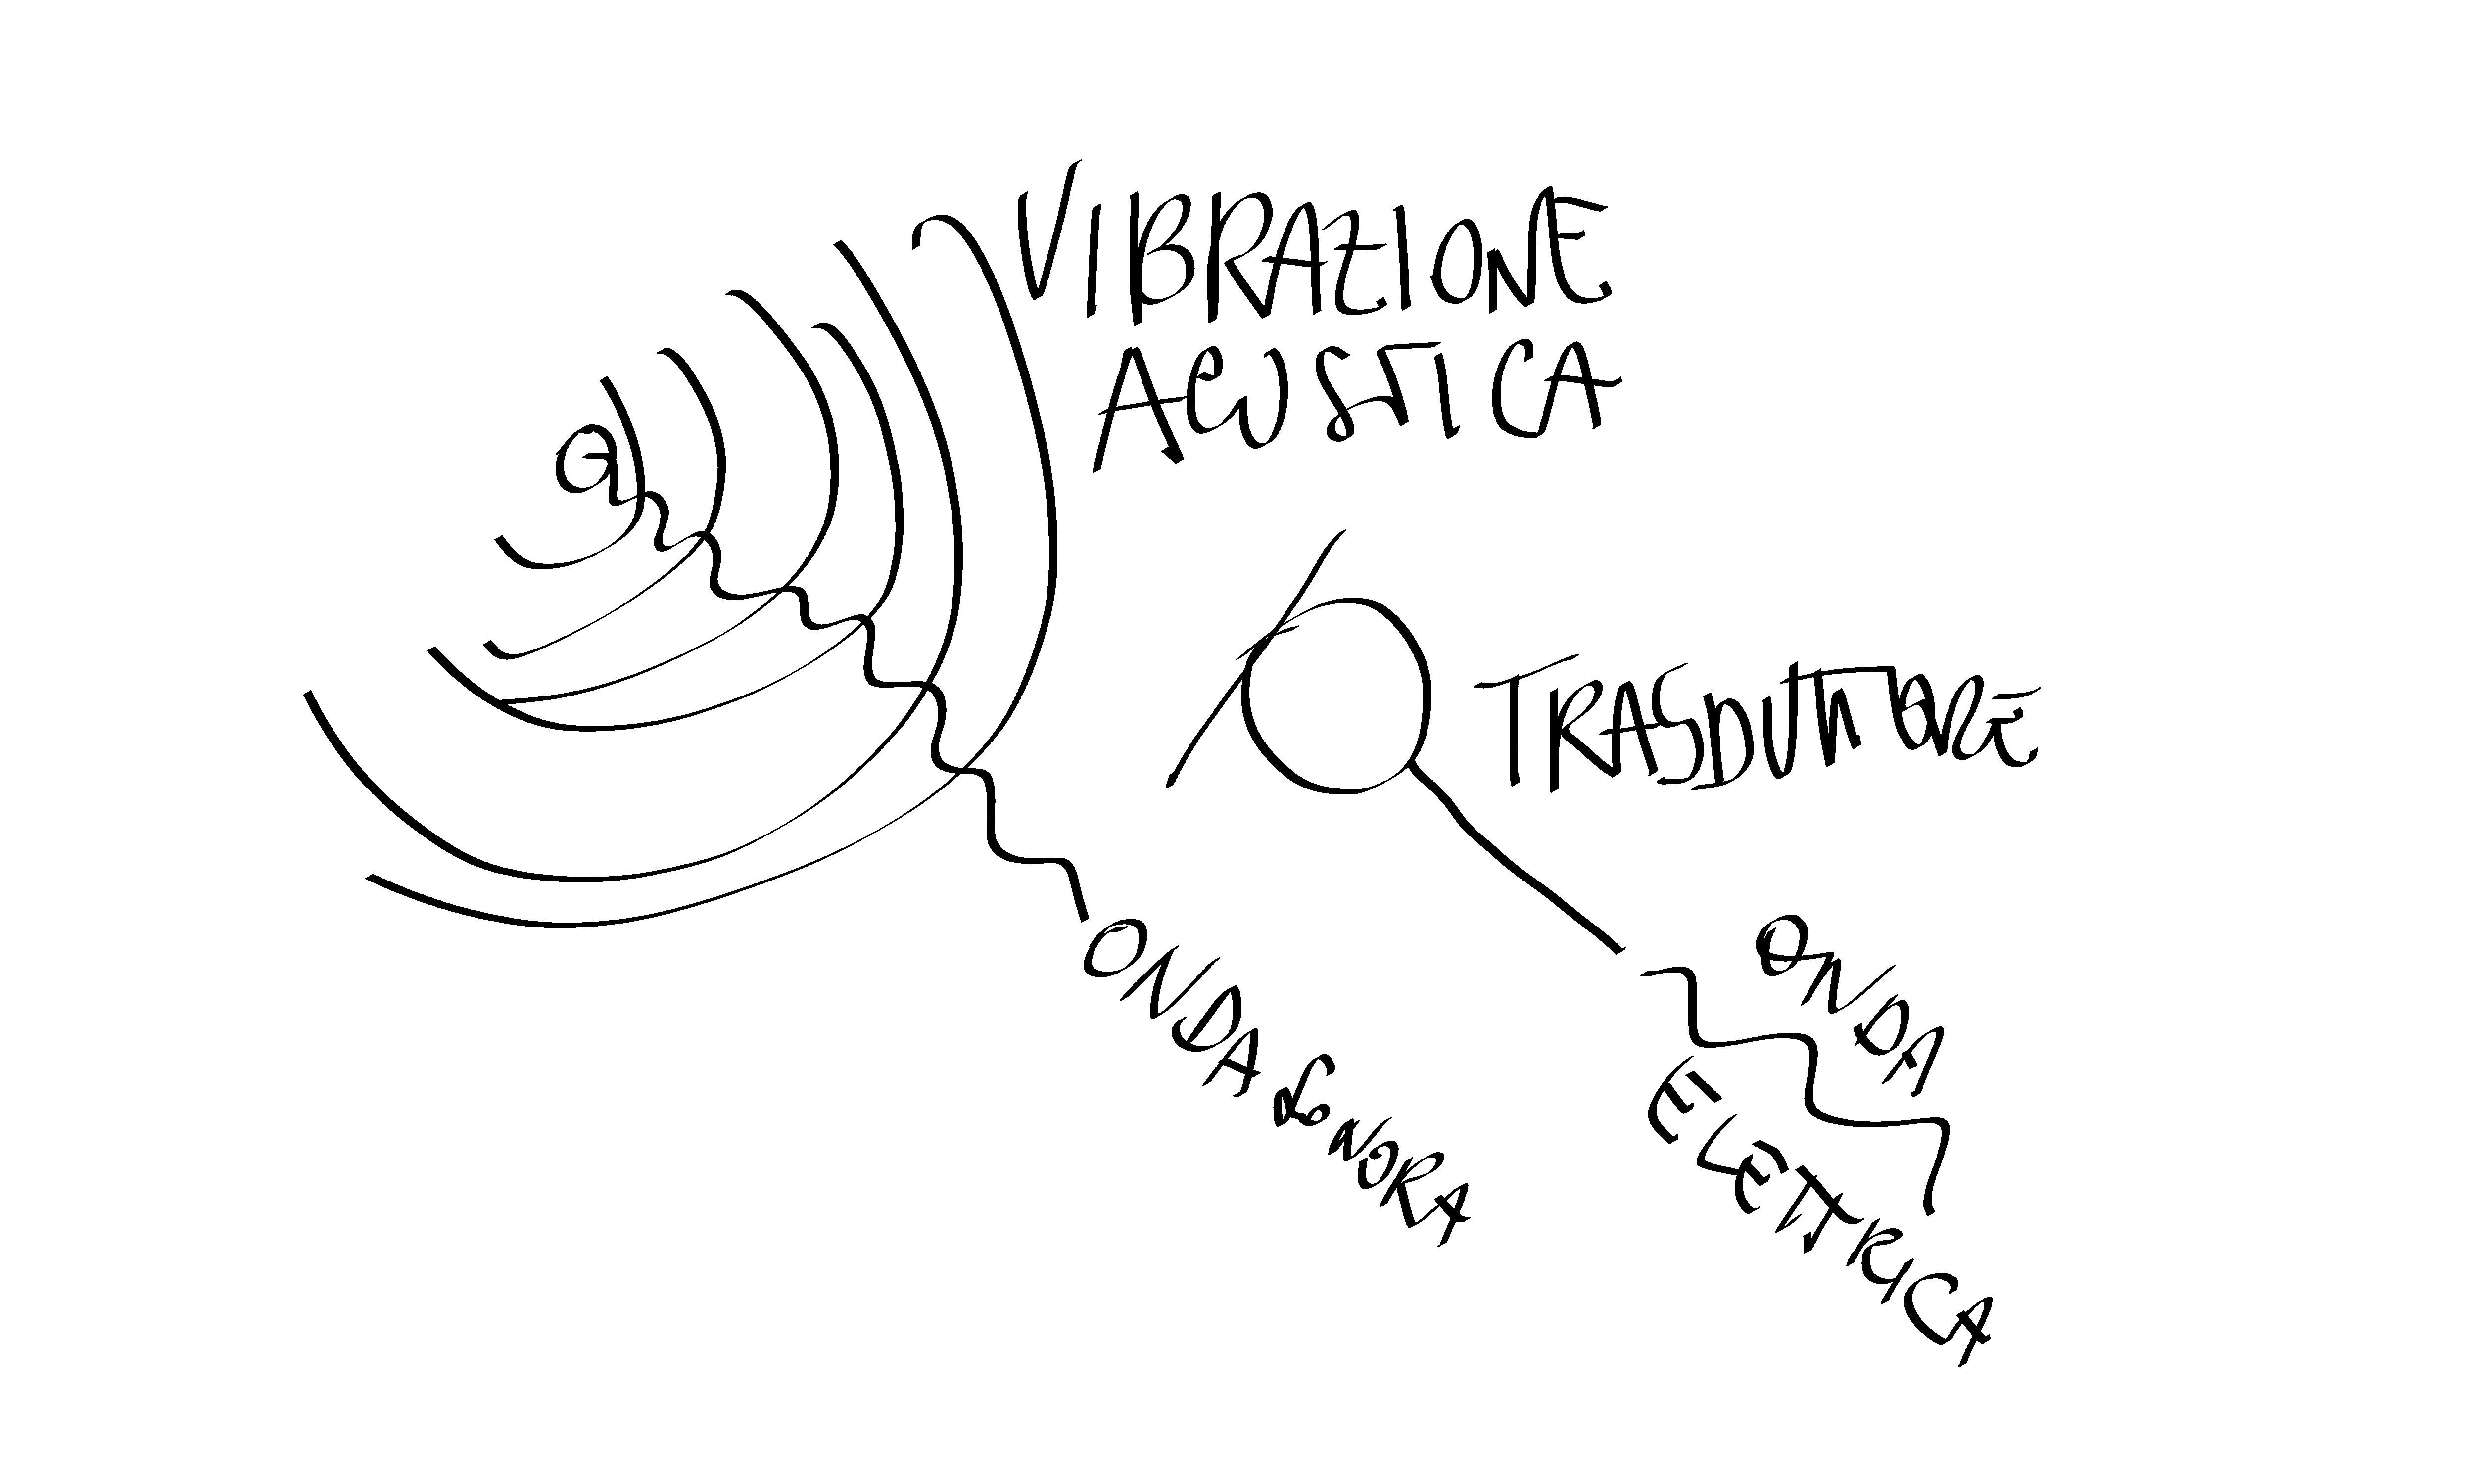
\includegraphics[width=0.99\columnwidth]{CAPITOLI/0200/img/trasduzione.png}
\caption[]{Generalizzazione di un sistema microfonico.}
\label{mic:condensatore}
\end{figure}

La generalizzazione del un microfono consiste in un sistema meccanico mobile esposto
all’onda sonora e destinato ad operare la \emph{trasduzione}\footnote{La
trasformazione della natura di un segnale operata da un trasduttóre,
derivato dall'inglese \emph{transducer} (che opera una trasduzione), dal latino
\emph{trans-ducere} (tras-portare). Il termine indica un dispositivo che converte
un segnale di data natura (acustica, elettrica, meccanica, termica, ecc.) in un
segnale di natura diversa. Si usa qualificare i t. con un aggettivo composto,
di cui la prima parte precisa la natura del segnale applicata e la seconda
parte quella del segnale d'uscita: t. acustoelettrico, che converte un suono in
un segnale elettrico (per es., un microfono), t. elettroacustico, da segnale
elettrico a suono (per es., un altoparlante). \\ – Fonte: Enciclopedia Treccani}
di una grandezza acustica, come la variazione di pressione, attraverso l'analogo
movimento meccanico rappresentato dallo spostamento della parte mobile del microfono, e da un sistema
elettrico a esso collegato destinato a operare la \emph{trasduzione} della
grandezza meccanica in una grandezza elettrica generando una una variazione di
corrente.

\begin{figure}[t!]
\centering
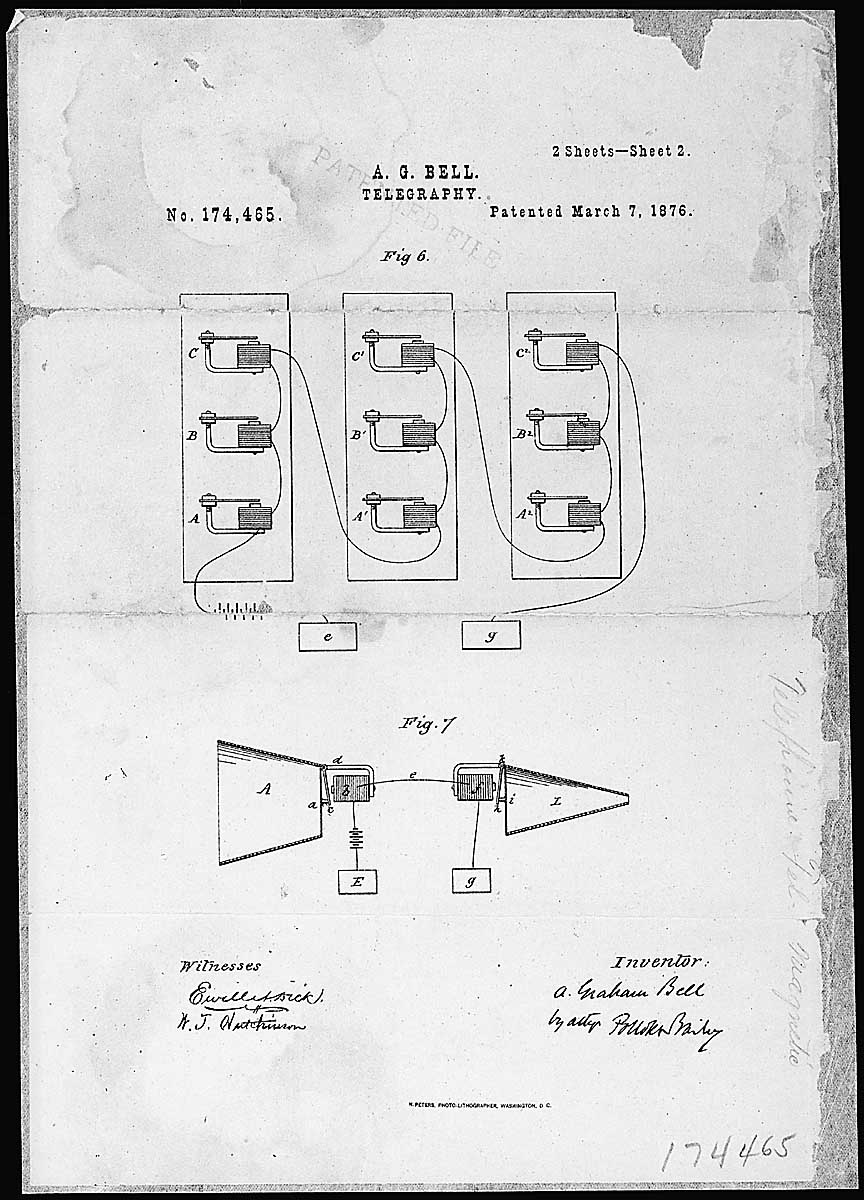
\includegraphics[width=0.99\columnwidth]{CAPITOLI/0200/img/telephone-patent-drawing-l.jpg}
\caption[]{Alexander Graham Bell.\\ Telegrafo. Registro brevetti: 302052.}
\label{agb:tel}
\end{figure}

Tutti i microfoni si attivano attraverso una specifica amplificazione elettrica,
motivo per cui potremmo dire che li alimentiamo per copiare il campo sonoro
piuttosto che prenderne energia, sottolineando però la peculiarità dell'osservazione
fisica: copiare il campo sonoro, intralciandolo.

Per qualche generazione si potrà parlare ancora del \emph{gioco del telefono}. Muovere
un messaggio sottovoce tra file di orecchie e bocche allo scopo di tras-portare
l'informazione, sperando che questa venga tras-figurata, tra le risate. Più
felici di così solo con l'esperimento di collegare tra loro due bicchieri di carta con
uno spago per parlarsi, sottovoce, a breve distanza. È il suono mobile, nel tempo
e nello spazio, il meccanismo del suono in viaggio, che ha reso tutto possibile.

\begin{figure}[t!]
\centering
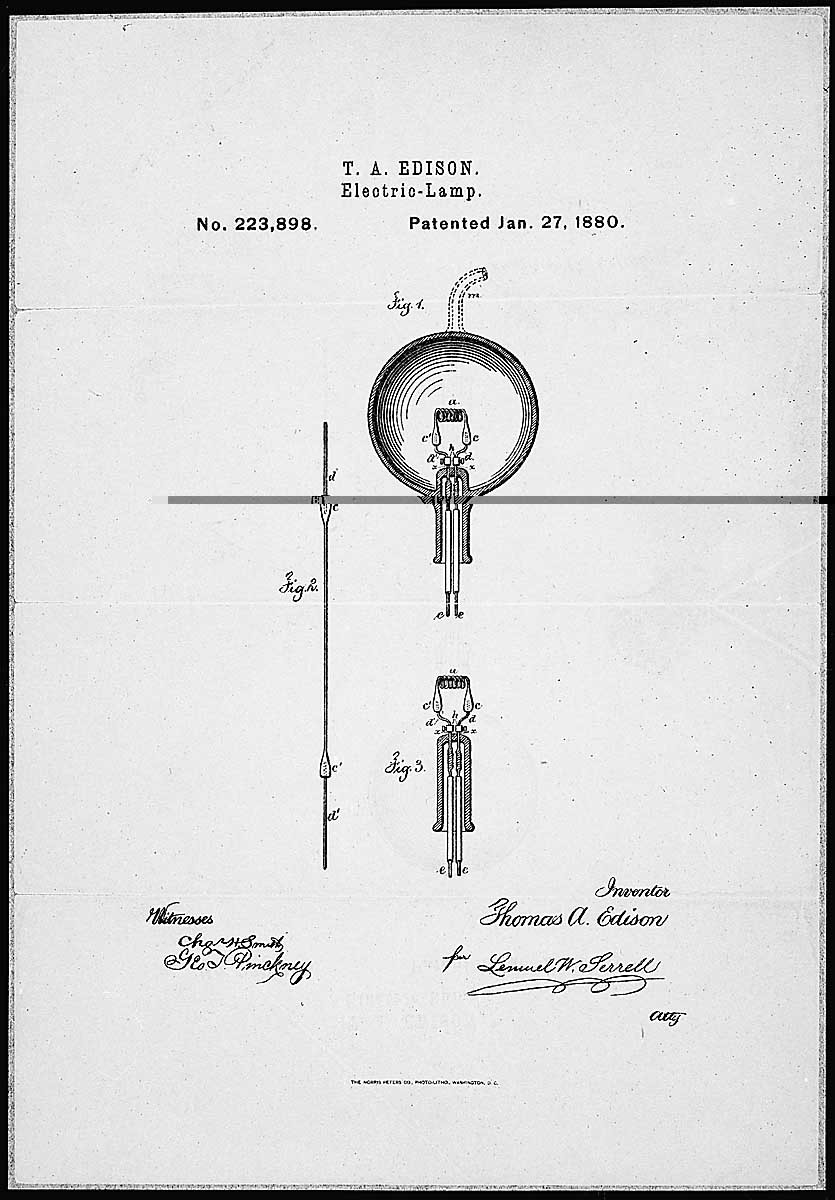
\includegraphics[width=0.99\columnwidth]{CAPITOLI/0200/img/light-patent-drawing-l.png}
\caption[]{Thomas Edison. \\ Lampada elettrica. Registro brevetti: 302053.}
\label{te:lamp}
\end{figure}

Nel 1876, a Philadelphia, si teneva la \emph{Centennial Exhibition} per celebrare
il centenario della nascita della nazione. Fu la prima fiera mondiale a tenersi
negli Stati Uniti con lo scopo, tra gli altri, di annunciare a tutti che la nazione era
ufficialmente una potenza industriale. All'interno degli edifici della fiera erano
esposte le opere di due inventori: Alexander Graham Bell e Thomas Alva Edison.

Un passo ulteriore nello sviluppo della modulazione in aria (senza contatto) della
corrente continua è stato sviluppato nel 1878 da David Edward Hughes. In quella
realizzazione delle barrette di carbonio fissate ai due estremi venivano messe in
vibrazione dalle onde sonore dando luogo a una fluttuazione abbastanza grande
della resistenza
di contatto tra l'asta di carbonio e i due punti di fissaggio. Questo tipo di
microfono fu impiegato da Clement Ader nel 1881 nella sua pioneristica trasmissione a due
canali dal teatro dell'Opera di Parigi al padiglione espositivo.
Fu Hughes, per inciso, a usare per primo il termine \emph{microfono}, applicato
ai dispositivi di questo tipo.

Furono le compagnie radio-televisive a spingere nello sviluppo di queste tecnologie,
fin dagli anni venti, per aumentare la qualità del suono elettroacustico ad
entrambi gli estremi della catena: microfoni ed altoparlanti.

La compagnia \emph{Western Electric}, il ramo produttivo della \emph{Bell Telephone},
rispondendo alle esigenze crescenti, sviluppava sia microfoni elettrodinamici che
a condensatore. Contemporaneamente in Europa Eugen Reisz stava cercando con George Neumann,
suo collaboratore, un nuovo sensore per avere un suono migliore rispetto al
microfono a dischi di carbone utilizzato nella telefonia. Le ricerche portarono alla
costruzione di un contenitore rettangolare fresato in un blocco di marmo o in
bachelite riempito di uno strato di finissimi granuli di carbone chiusi da un
diaframma non conduttore. L’involucro in marmo risulta privo di risonanze e la
cavità con i granuli di carbone è sigillata costituendo un \emph{microfono dinamico a pressione}.

\begin{figure}[t]
\centering
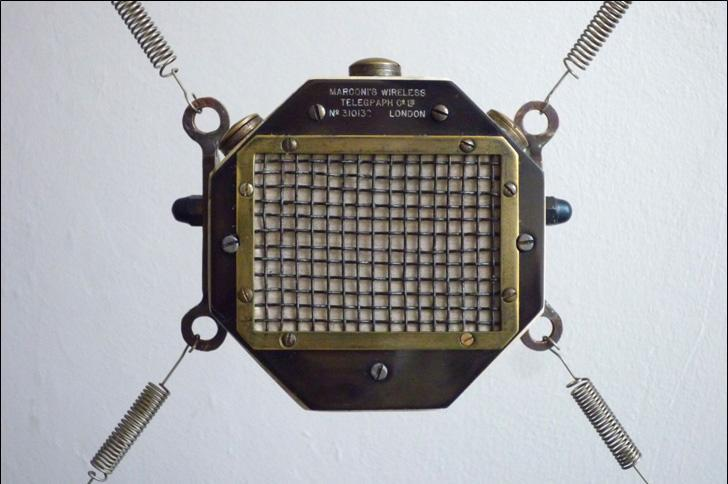
\includegraphics[width=0.99\columnwidth]{CAPITOLI/0200/img/1321872621718Reisz8.jpg}
\caption[]{Microfono \emph{Marconi-Reisz}, restauro RAI.}
\label{mic:Marconi-Reisz}
\end{figure}

Il microfono, progettato in Germania, è stato prodotto nel Regno Unito nel 1925/26
dalla \emph{Marconi Wireless}, motivo per cui è conosciuto come microfono
\emph{Marconi-Reisz} poi prodotto anche da \emph{AEG (Allgemeine Gesellschaft
Elektrik)} con piccole differenze costruttive. Aveva una risposta in frequenza da $50Hz$ ai $1000Hz$ in modo
piuttosto lineare, estendendosi meno linearmente fino ai $10KHz$. Un microfono
di notevole qualità per quell’epoca, molto sensibile, che quindi veniva montato su un supporto elastico.

La risposta in frequenza poteva essere migliorata ulteriormente attraverso un
circuito elettrico e qualche accorgimento operativo. Un'informativa interna
della \emph{BBC} del 1935 comunicava \emph{lo speaker deve
parlare attraverso il microfono ad un angolo di 45 gradi}, a sottolineare la relazione tuttora valida
tra dimensione del diaframma, angolo di incidenza e risposta in frequenza.
Le costruzioni successive portarono migliorie timbriche, nonostate alcune limitazioni
tra cui il livello di rumore di fondo abbastanza alto, causato dalle minuscole
scintille di scarica tra i granuli.
Un altro problema era che i granuli gravitavano verso il basso e
si compattavano. Questo produceva un livello di fruscio maggiore e una minore
sensibilità. Uno dei compiti dei tecnici audio dell’epoca era quello di passare
quotidianamente, e prima di ogni programma, negli studi e girare i microfoni
\emph{Reisz} a testa in giù e scuotendoli in modo da ridistribuire i granuli compattati.
Il manuale di Istruzioni del 1935 indicava che
il microfono doveva essere scollegato \emph{e, posto con il diaframma orizzontale
e rivolto verso l'alto\ldots} deve inoltre \emph{essere ben agitato da un lato all'altro in
modo da allentare il compattamento dei granuli}.

\subsection{Architettura e principio di funzionamento}

Nonostante in termini di principi generali ci sia solo modo, per ora, di
trasformare le onde acustiche (copiandone il movimento) in variazioni di tensione,
perdurano, fin dalla nascita di queste tecnologie, diversi modi per farlo.

Una prima catalogazione dei microfoni può essere effettuata per architettura,
ovvero in funzione delle caratteristiche costruttive che ne determinano i
risultati in termini di trasduzione.

In questa classificazione troviamo:

\begin{compactitem}
  \item microfoni dinamici
  \item microfoni a nastro
  \item microfoni a condensatore
  \item microfoni a condensatore electret
\end{compactitem}

\subsubsection{Microfoni dinamici}

Il microfono dinamico (indicato anche a bobina elettrodinamica,
elettromagnetica o mobile) si basa sul principio dell'induzione magnetica in cui
il conduttore, nel caso specifico l'avvolgimento di filo della bobina, si muove
attraverso un campo magnetico inducendo una tensione proporzionale alla forza
del campo magnetico, alla velocità del movimento e all'ampiezza del movimento
lungo il campo magnetico.

\begin{figure}[h]
\centering
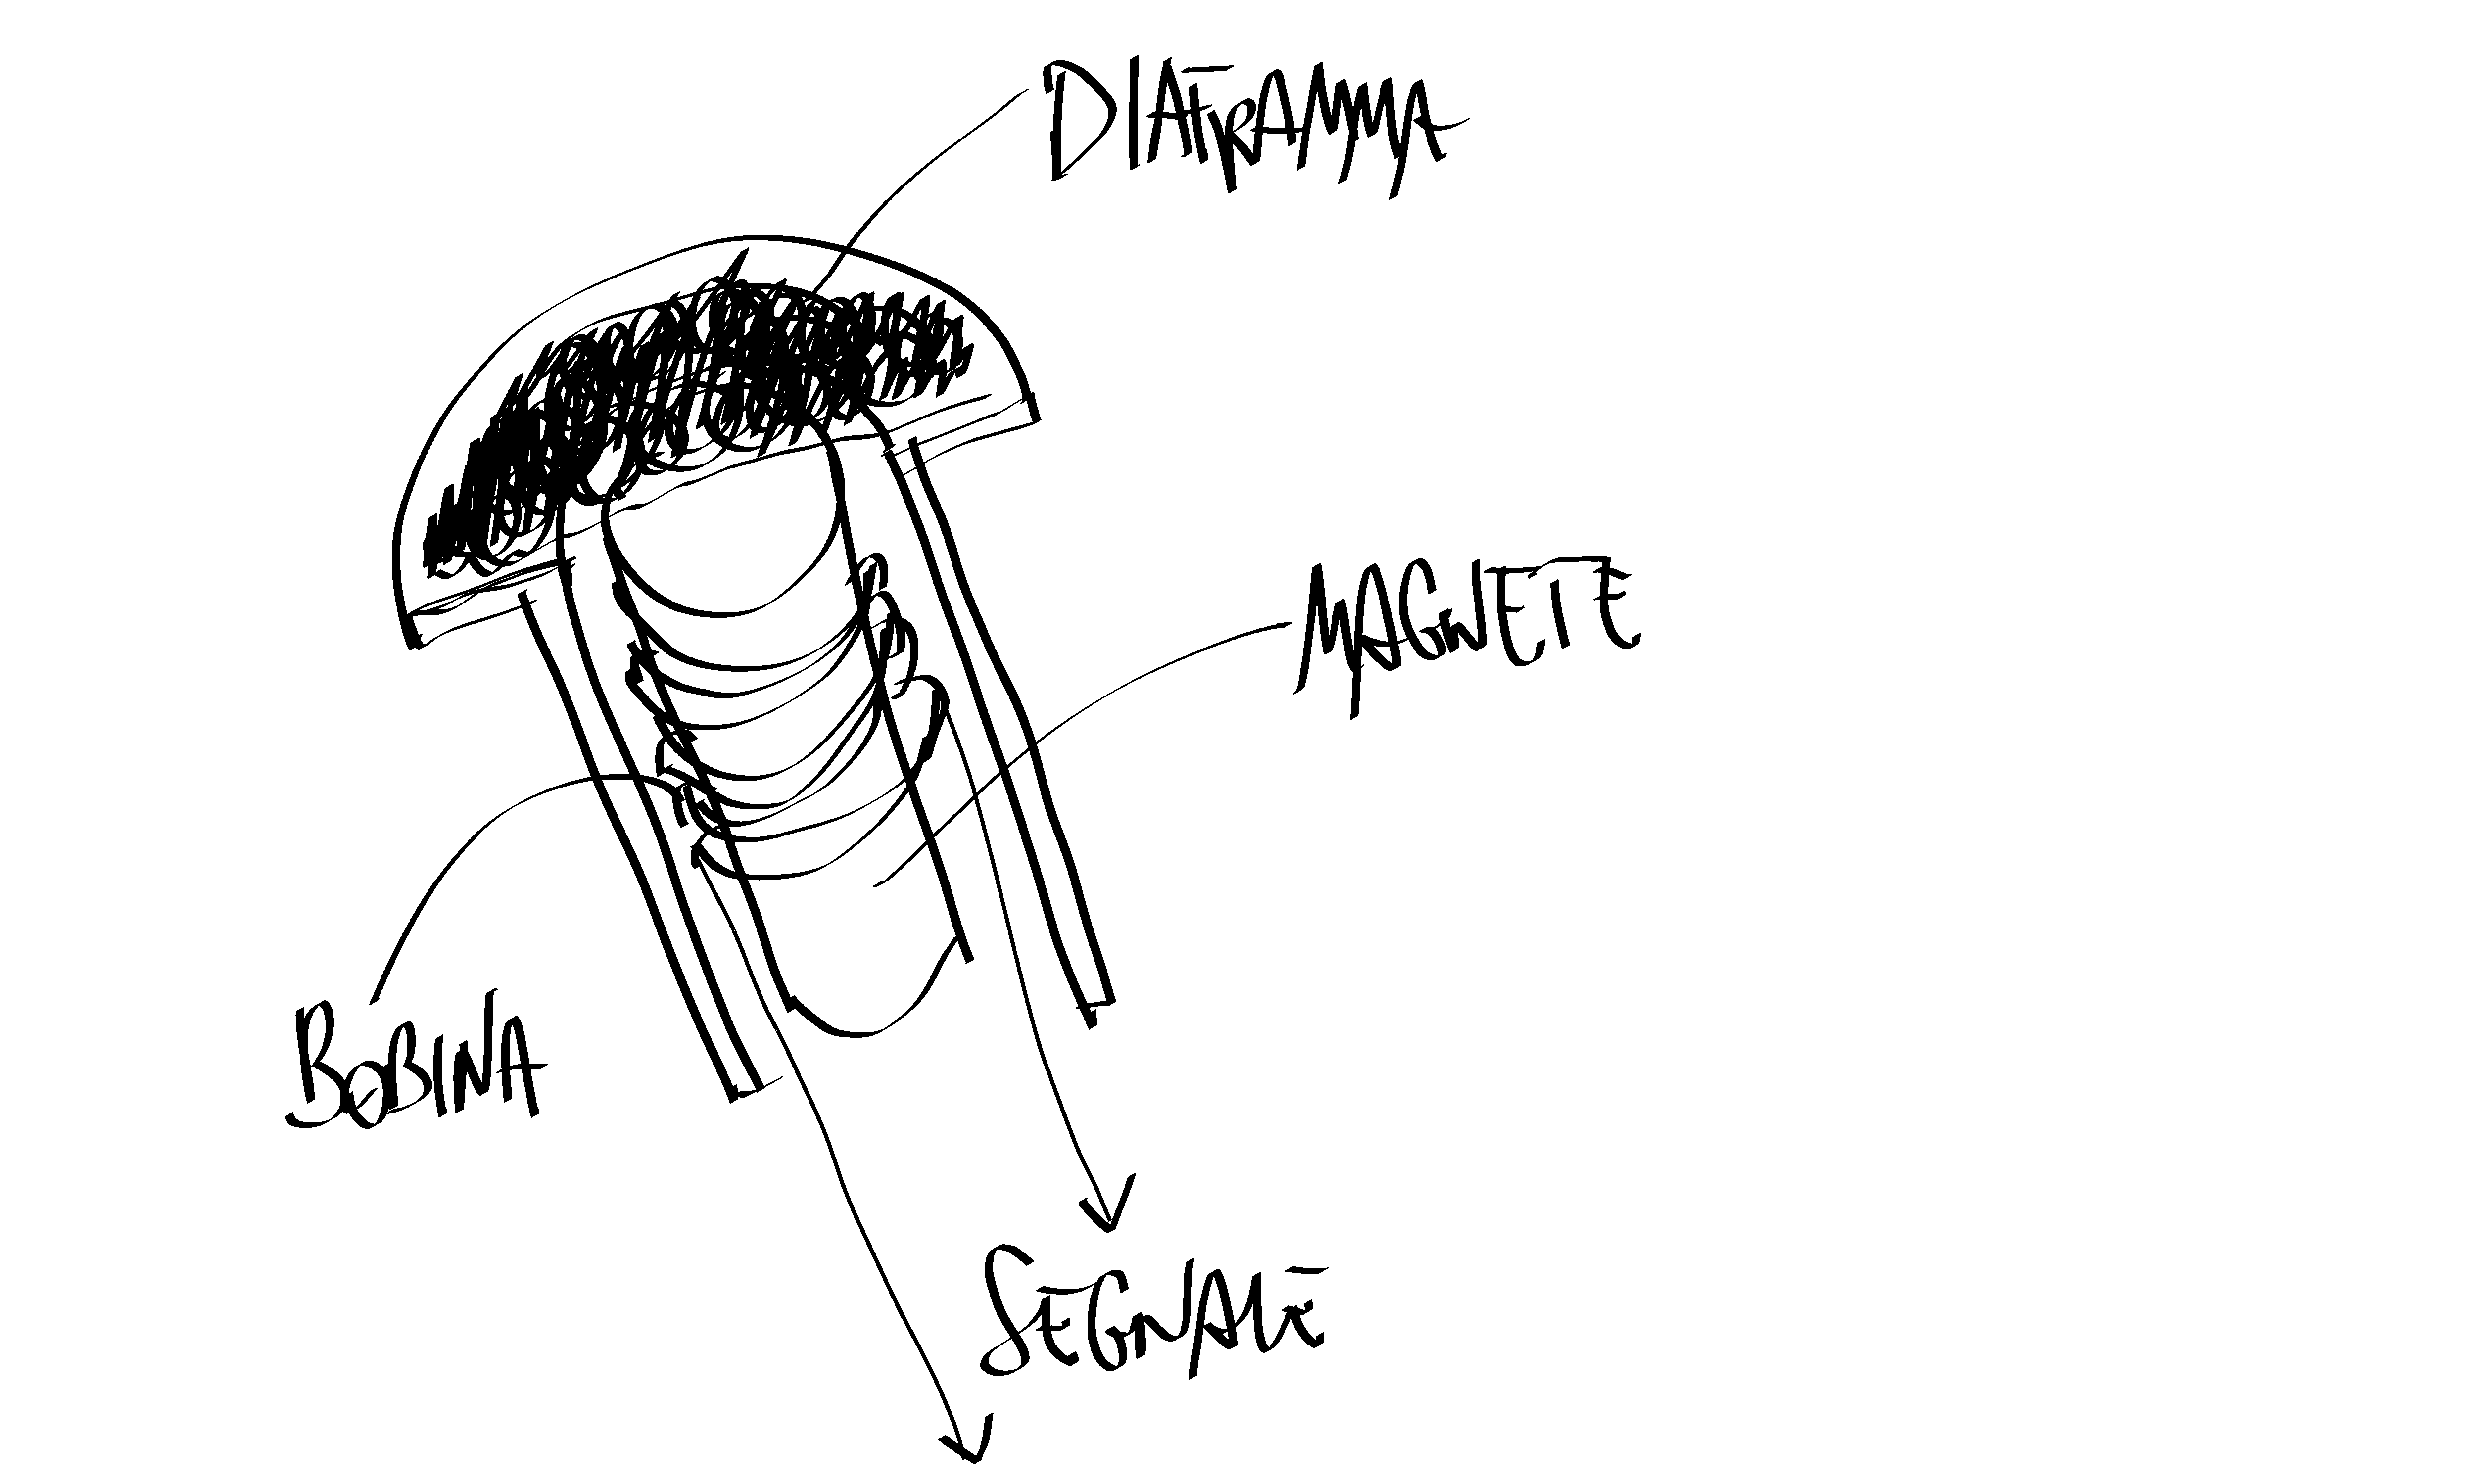
\includegraphics[width=0.99\columnwidth]{CAPITOLI/0200/img/mic-dinamic.png}
\caption[]{Microfono dinamico.}
\label{mic:dinamico}
\end{figure}

%A tale famiglia appartengono microfoni, la cui architettura è schematizzata in fig. 1,

Il diaframma circolare messo in vibrazione dalle onde sonore trasmesse nell’aria
è solidale con l'avvolgimento di filo di rame della bobina, libero di muoversi
all’interno di un campo magnetico costituito da un magnete permanente.

Le onde sonore, costituite da compressioni e rarefazioni dell’aria secondo una
determinata frequenza (corrispondente all’altezza del suono), vengono perciò
trasformate, attraverso tale trasduttore, in corrente elettrica, presente sui
cavi di uscita alle estremità dell’avvolgimento di rame, con variazioni di
ampiezza e frequenza analoghe a quelle delle onde acustiche. Questo
principio di trasduzione, come vedremo in seguito, non è altro che il
procedimento inverso a quello della maggior parte degli altoparlanti, nel qual
caso, una corrente elettrica proveniente dall’amplificatore si presenta ai
poli estremi di una bobina mobile, anch’essa libera di muoversi all’interno di
un campo magnetico, e genera una corrispondente vibrazione sul cono
dell’altoparlante solidale alla bobina.

Le caratteristiche salienti di questo tipo di microfono sono:

\begin{compactitem}
  \item estrema robustezza ed affidabilità
  \item segnale di uscita molto basso
  \item risposta rimbrica limitata in banda
  \item scarso rapporto tra segnale e rumore
\end{compactitem}

È importante osservare come, a causa dell’elasticità e della massa del materiale
vibrante, il gruppo diaframma-bobina abbia una sua frequenza di risonanza
caratteristica. Al di sotto di tale frequenza il comportamento è dettato dal
rapporto elasticità/rigidità, mentre al di sopra dipende dalla massa del
complesso vibrante. Questo è uno dei motivi per cui i microfoni dinamici
tendono a \emph{colorare} il suono quando l'altezza in entrata si muove attorno
alla frequenza di risonanza, e tendono ad avere anche una risposta non perfettamente
estesa alle alte frequenze, a causa dell’inerzia delle masse in movimento.

Il rapporto tra qualità del segnale è proporzionale al numero degli avvolgimenti
della bobina, per cui il vantaggio della riduzione delle masse vibranti è
controbilanciato da un segnale di uscita inferiore, con conseguente diminuzione
del rapporto segnale/rumore. La soluzione risiede nel compromesso tra i valori
ottimali di tutti questi parametri.

L'evoluzione dei materiali nel campo dell'elettroacustica ha portato l'introduzione
nei sistemi dinamici (magnetici) del neodimio, utilizzato sia nei sistemi di
diffusione che di ripresa. La qualità del neodimio è nell'essere un materiale ad
alta coercitività, consentendo l’utilizzo di bobine a massa ridotta, a tutto
vantaggio della risposta alle alte frequenze.

\subsubsection{Microfoni a nastro}

In questo tipo di microfono il principio di funzionamento è assimilabile a
quello del microfono dinamico, con la differenza che la parte vibrante non è
costituita da un diaframma solidale ad una bobina mobile, bensì è costituito
da un sottilissimo foglio di alluminio
ondulato, anch’esso libero di vibrare tra i poli di un magnete permanente, e
alle estremità del quale si produce una tensione elettrica derivante dalle
onde sonore in entrata. In questo tipo di microfono le funzioni
di vibrazione e di trasduzione sono svolte dallo stesso elemento fisico.

\begin{figure}[h]
\centering
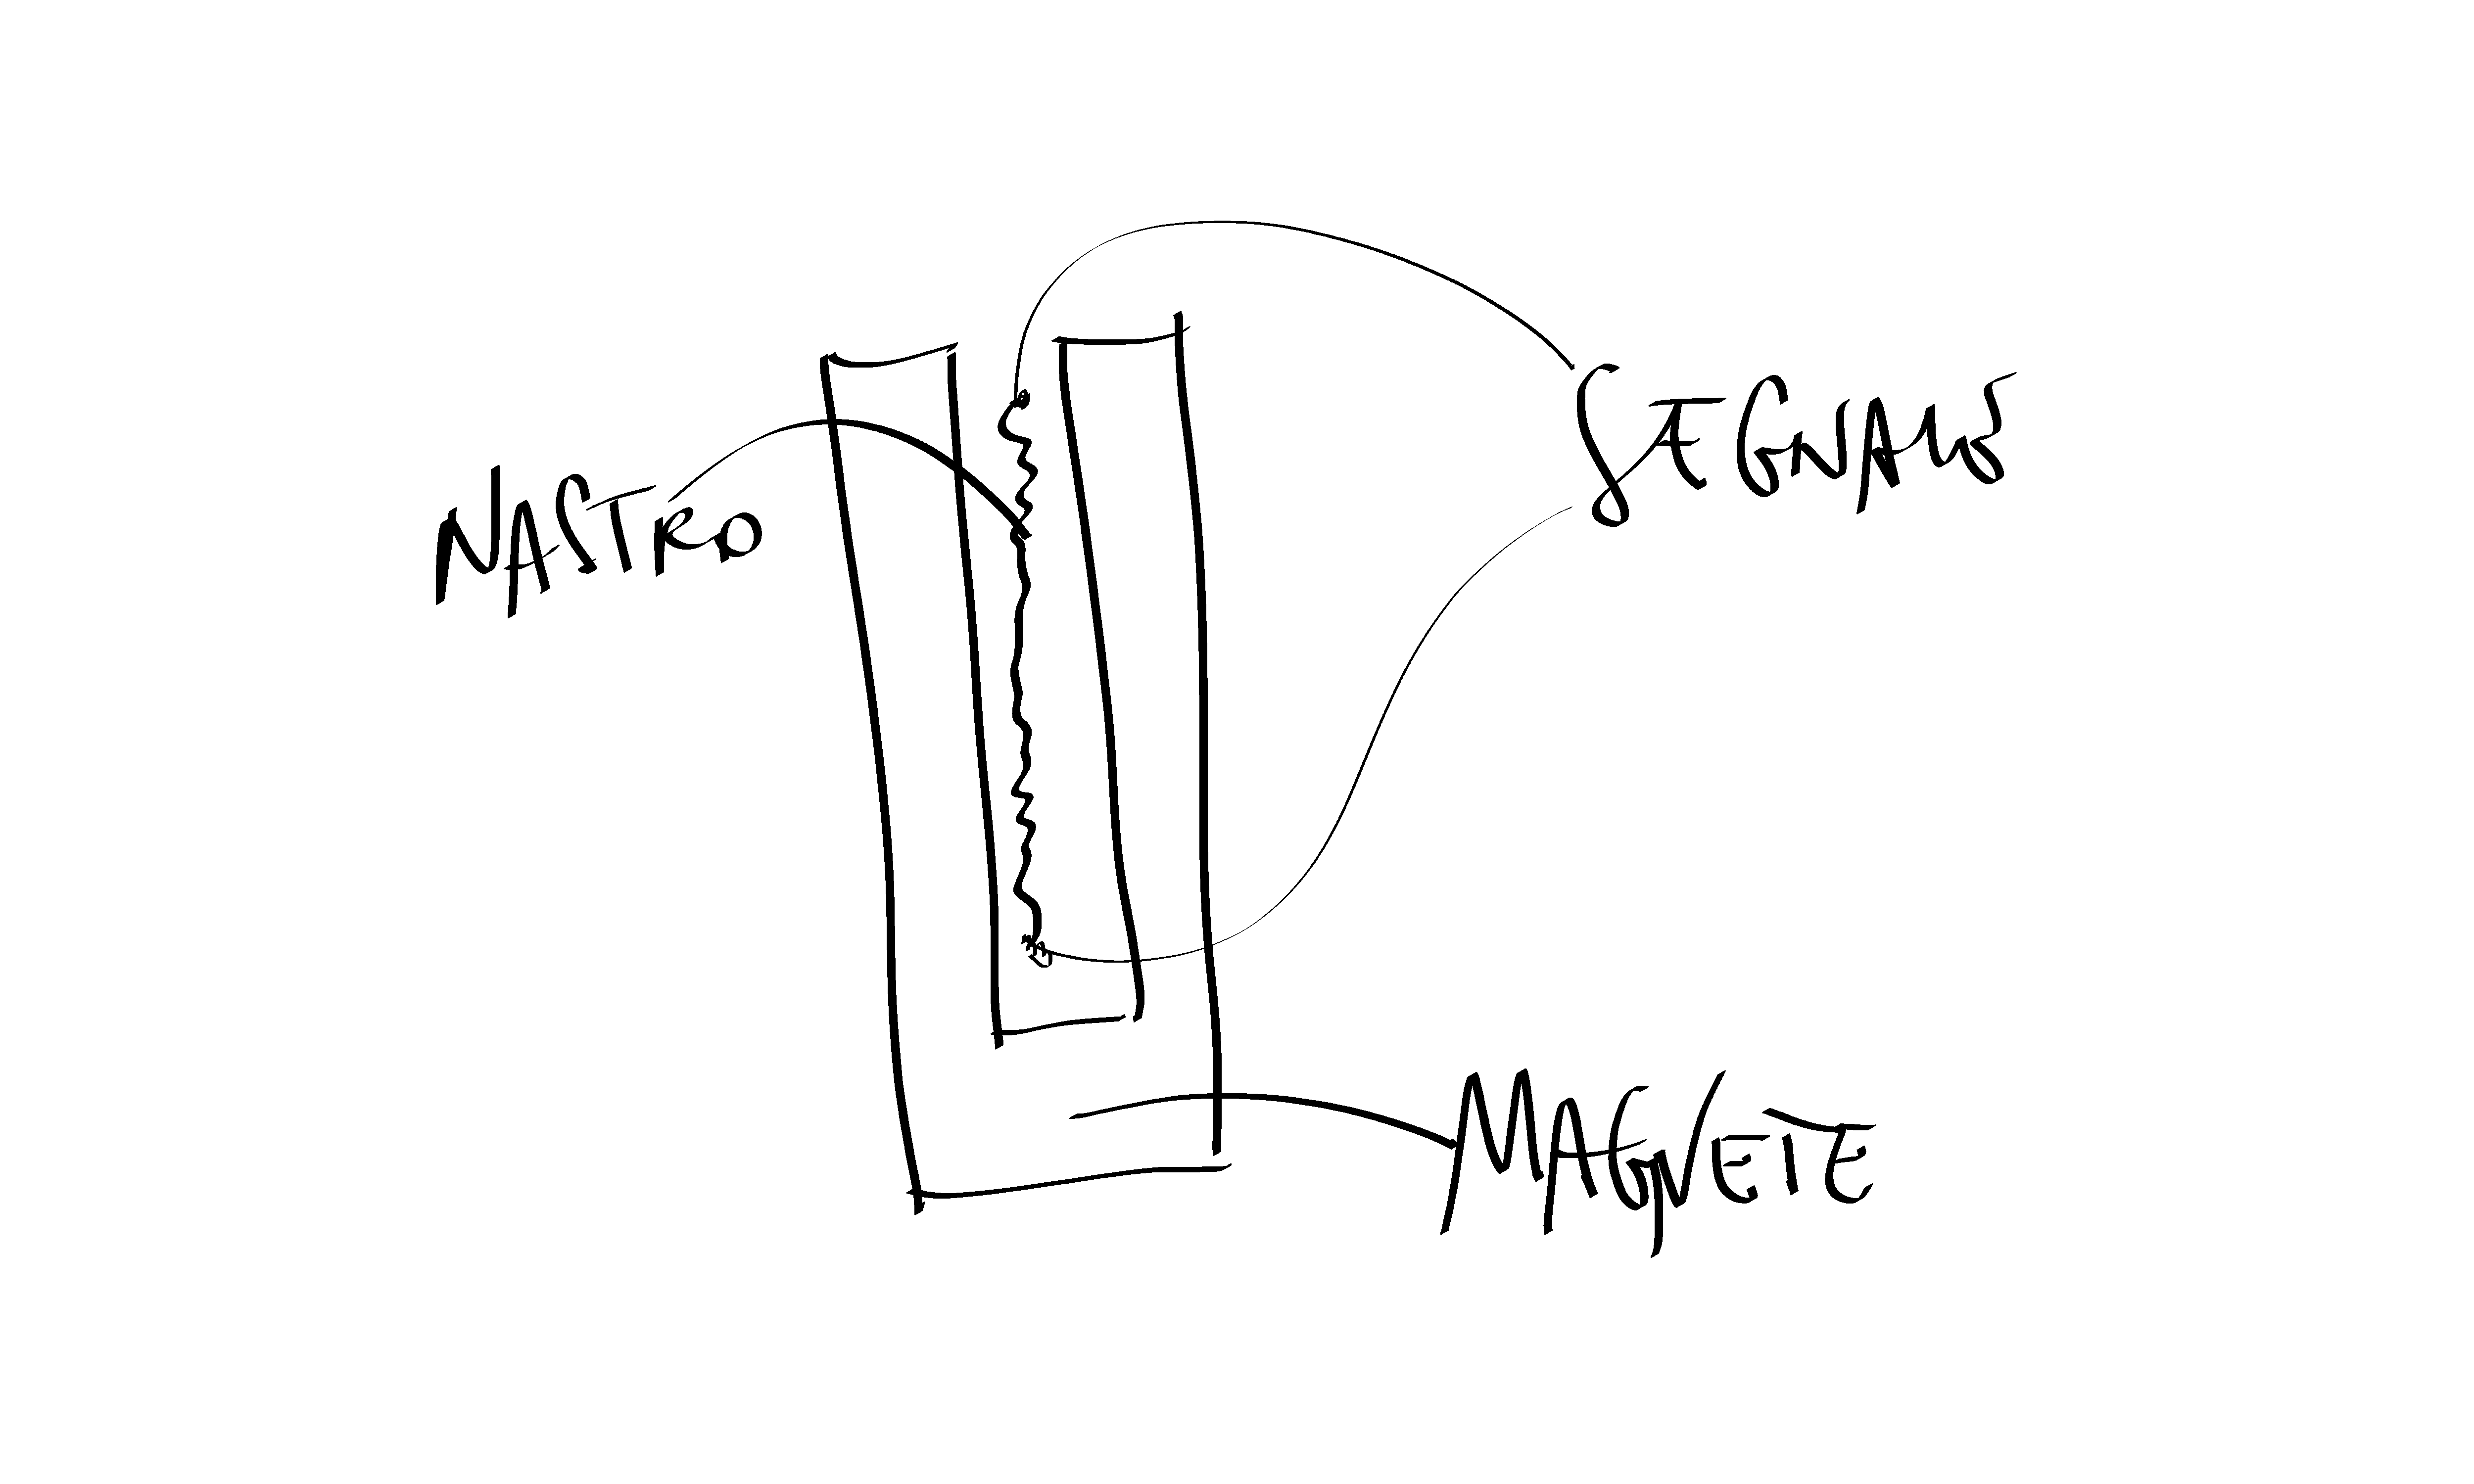
\includegraphics[width=0.99\columnwidth]{CAPITOLI/0200/img/mic-nastro.png}
\caption[]{Microfono a nastro.}
\label{mic:nastro}
\end{figure}

I primi microfoni a nastro erano piuttosto grandi, con magneti pesanti ed
inefficienti. Inoltre era piuttosto conosciuta la fragilità del nastro.

Le caratteristiche timbriche del microfono a nastro sono:

\begin{compactitem}
  \item assenza di coloratura dovuta alla frequenza di risonanza situata molto
  più in basso rispetto ai microfoni dinamici (inferiore ai $40Hz$);
  \item risposta estesa sulle alte frequenze a causa della ridotta massa del
  diaframma vibrante.
\end{compactitem}

Il segnale d’uscita prodotto ha generalmente un livello estremamente basso,
ed essendo bassa anche l’impedenza di uscita, viene interposto un trasformatore
per elevarlo di intensità e fornire un’impedenza conforme ad un segnale microfonico standard.

La sottigliezza del nastro vibrante può essere causa di fragilità del dispositivo,
rendendolo inadatto alla microfonazione di segnali dotati di un’elevata pressione
sonora. Caratteristica di questo tipo di microfono è la naturale risposta bi-polare,
denominata figura-8, che sarà meglio descritta in seguito.

\subsubsection{Microfoni a condensatore}

Edward Christopher Wente iniziò a lavorare per la \emph{Western Electric} nel 1914
sullo sviluppo oe la calibrazione di un
trasmettitore (o microfono) uniformemente sensibile per usi di laboratorio.
I microfoni a disco di carbone utilizzati nei ricevitori telefonici avevano una
risposta in frequenza troppo stretta, irregolare e un rumore di fondo eccessivo
per poter essere applicati nella ricerca sul suono. Con l'utilizzo
dell'amplificatore valvolare di Harold Dean Arnold, nel 1916, Wente produsse il
primo microfono a risposta in frequenza piatta da lui denominato trasmettitore a
condensatore. L'anno successivo pubblicò i suoi risultati in
un articolo teorico su \emph{The Physical Review}. Nel 1922, produsse un
trasmettitore a condensatore con una sensibilità cento volte maggiore, il che
era abbastanza per renderlo un dispositivo pratico, sebbene la sua alta
impedenza richiedesse il collegamento diretto ad un preamplificatore valvolare.

Il microfono a condensatore moderno è molto simile ai modelli originari di Wente
del 1917, solo molto più piccoli e raffinati nella costruzione. Spesso  in lingua
inglese ci si riferisce a tale microfono attraverso il termine
\emph{condenser microphone}, tuttavia il termine rivela delle ambiguità e già
dagli anni venti del novecento ci si è riferiti con più precisione alla tecnologia nei termini
di \emph{capacitor microphone}.

\begin{figure}[h]
\centering
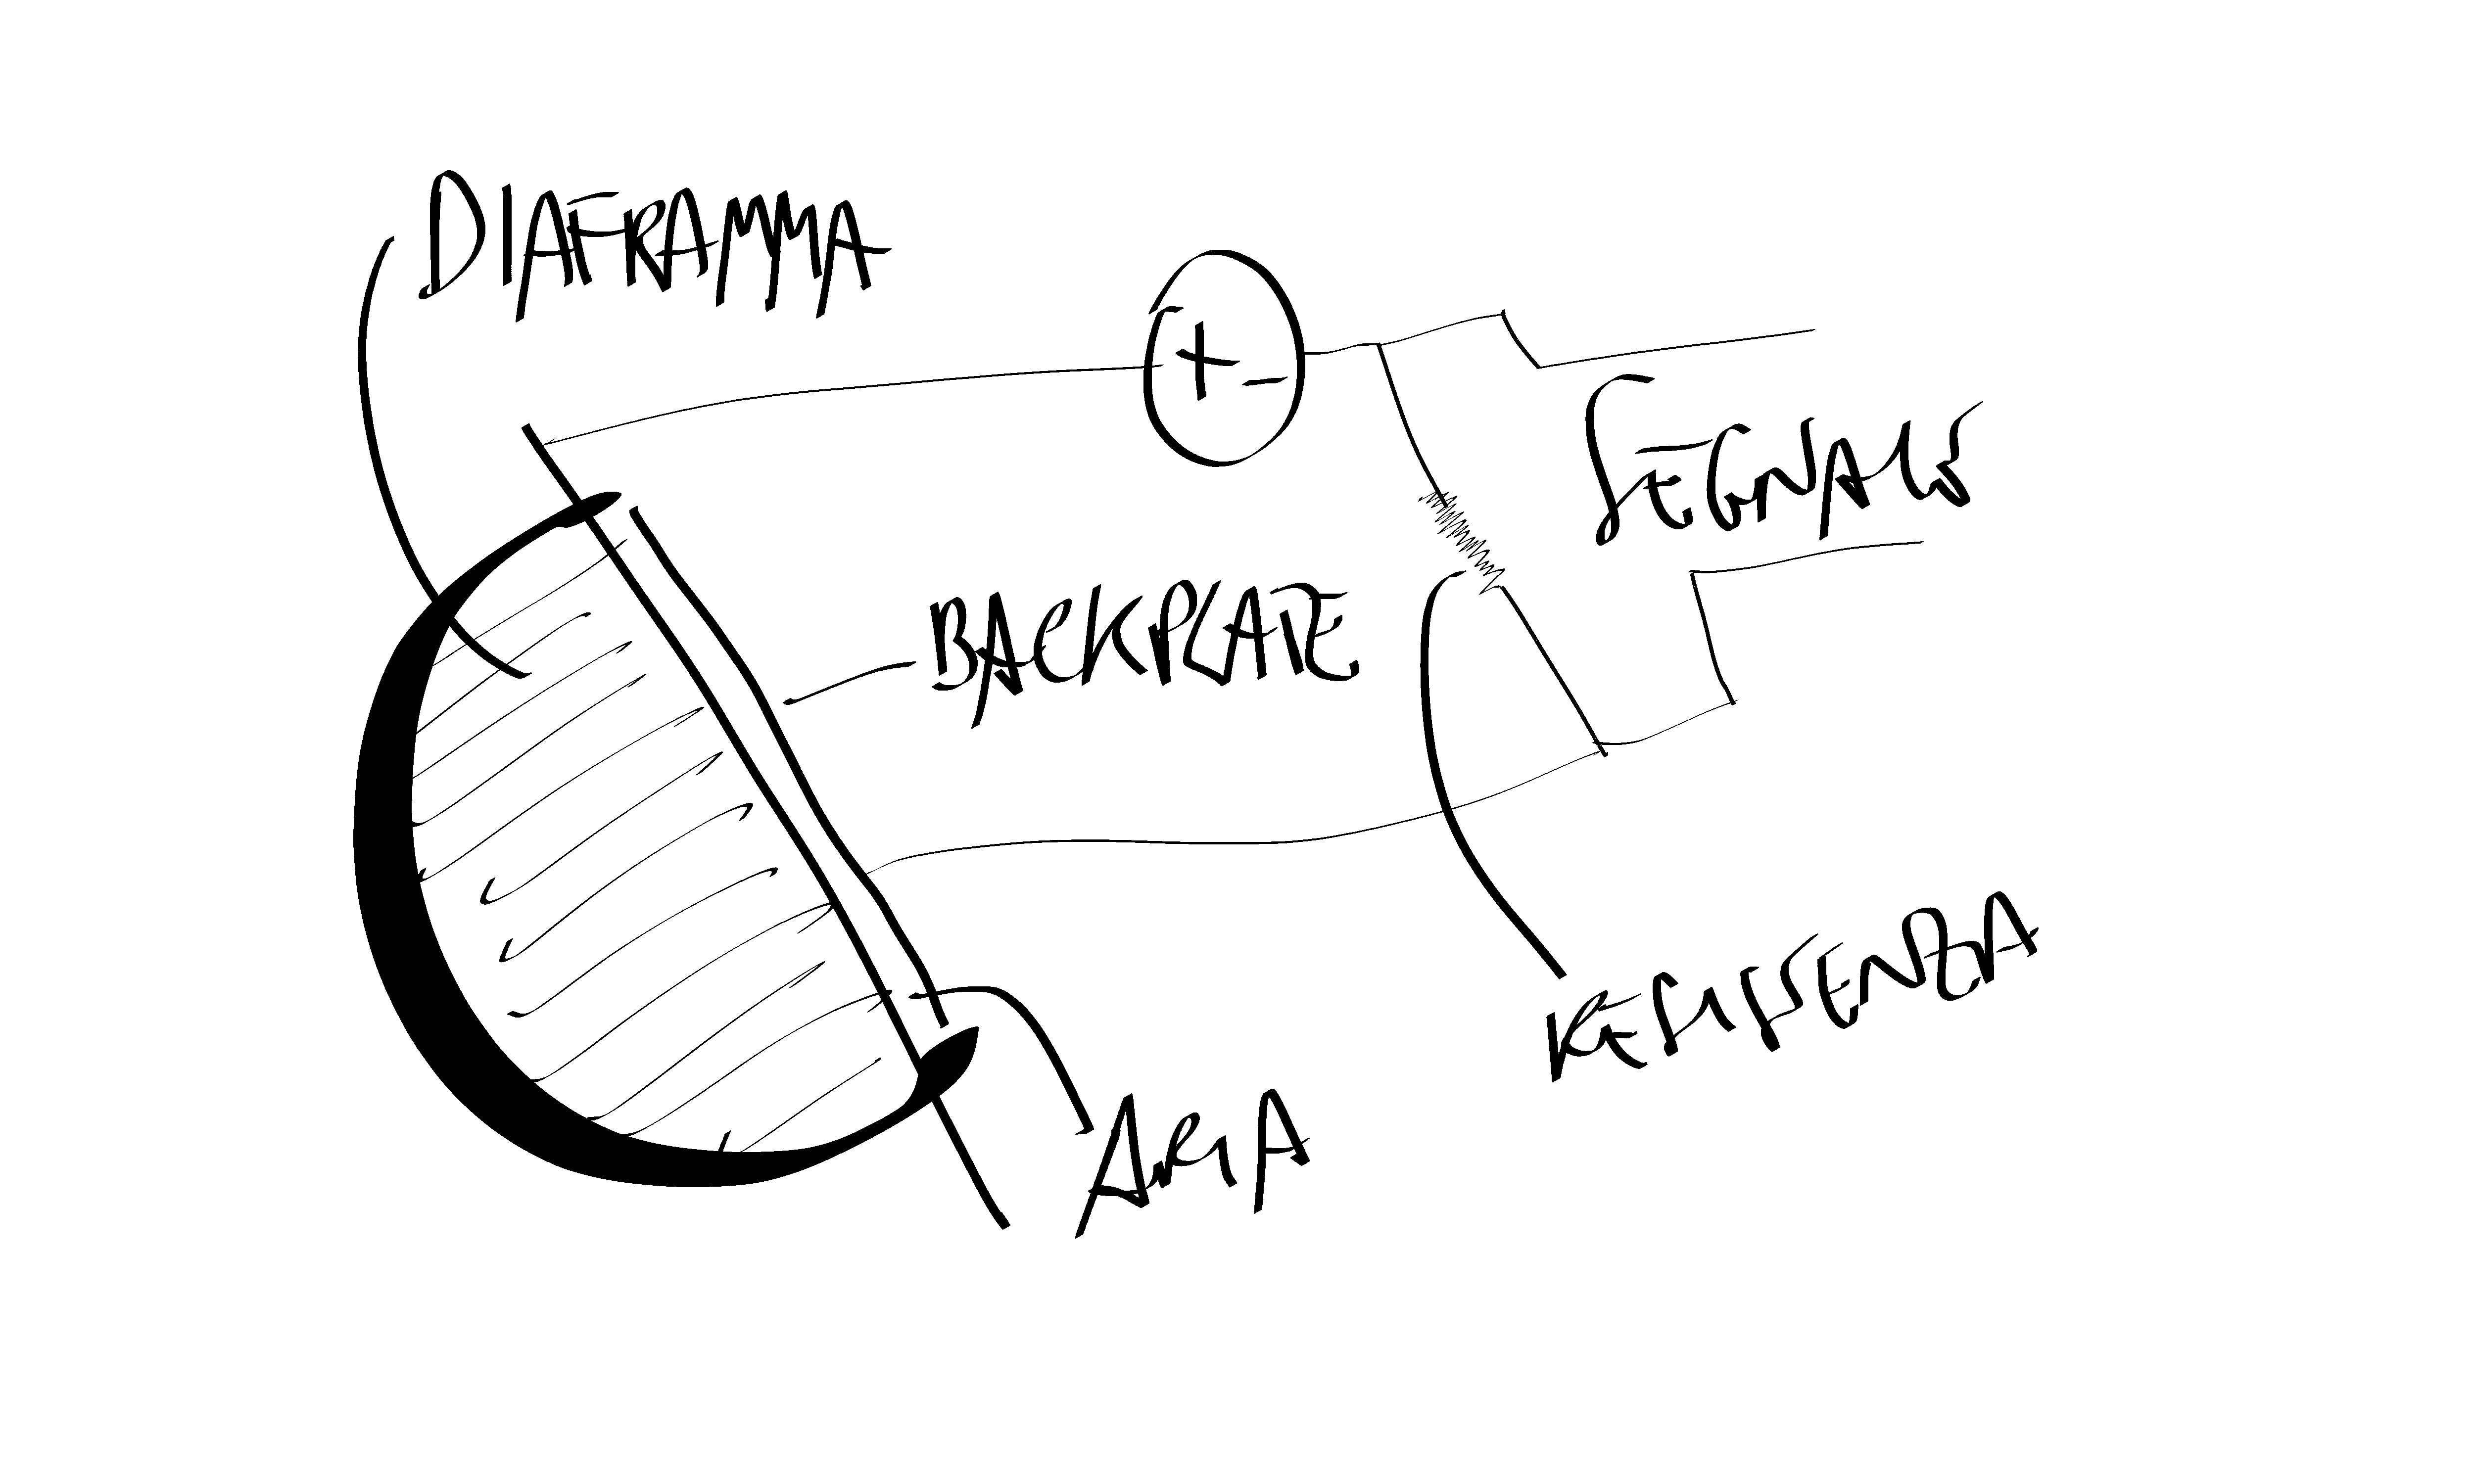
\includegraphics[width=0.99\columnwidth]{CAPITOLI/0200/img/mic-capacitor.png}
\caption[]{Microfono a condensatore.}
\label{mic:condensatore}
\end{figure}

Il microfono a condensatore è costituito da un diaframma (solitamente in materiale
plastico o metallico molto leggero come alluminio, nickel e titanio)
rivestito finemente d'oro. La lamina è distanziata da una seconda lamina fissa, più spessa,
denominata \emph{backplate} (lamina posteriore) che può essere forata. Le due
lamine hanno tra loro una differenza di potenziale in quanto
viene applicata esternamente una tensione di polarizzazione in corrente continua ad una delle
due.

\begin{figure}[tbhp]
\centering
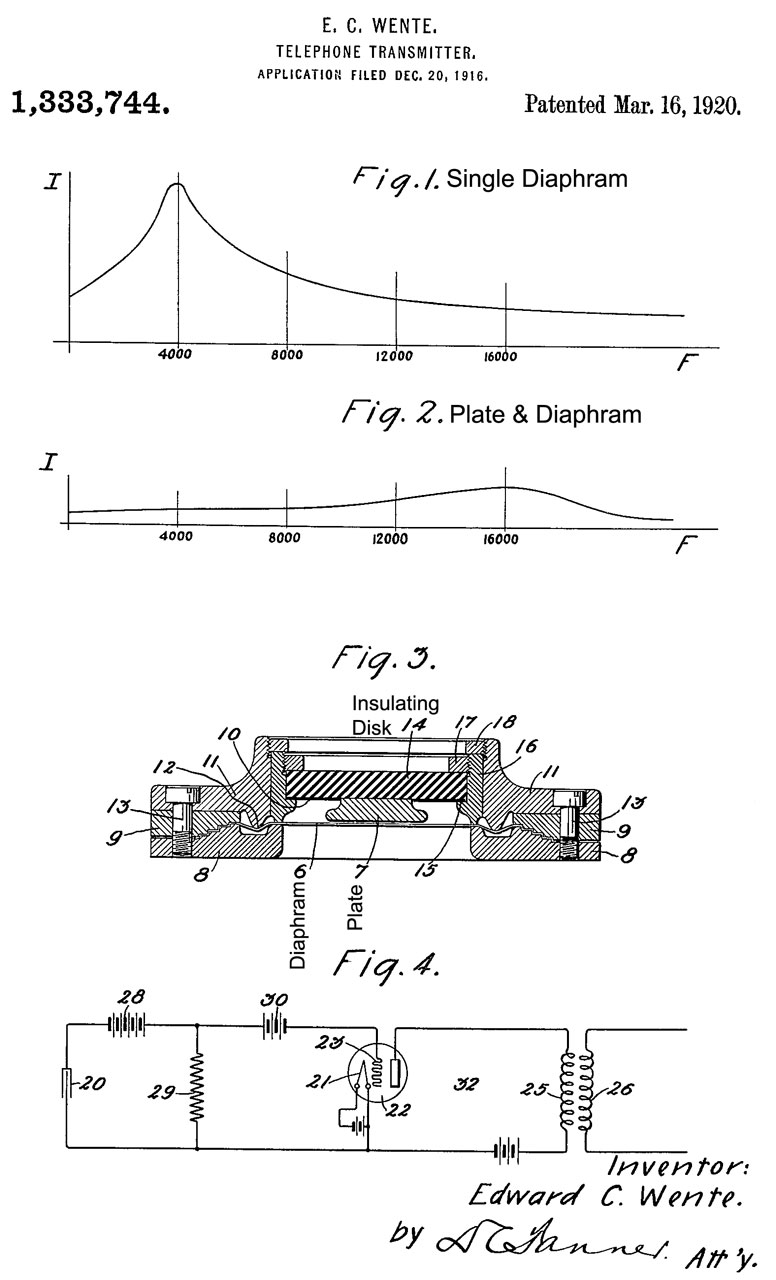
\includegraphics[width=0.99\columnwidth]{CAPITOLI/0200/img/US1333744-1b.jpg}
\caption[]{Edward Christopher Wente. \\ Microfono a condensatore. Registro brevetti: 1333744.}
\label{mic:wentemic}
\end{figure}

Il condensatore è un elemento elettronico passivo pre-polarizzato, in grado di
bloccare il passaggio di corrente alternata attraverso i conduttori tra i quali
è posizionato un diverso tipo di dielettrico. Quando esiste una differenza di
potenziale (tensione) tra i conduttori, viene generato un campo elettrico
statico che viene separato dal dielettrico tra cariche positive e negative
memorizzate rispettivamente sul polo positivo e negativo del condensatore.

Secondo il principio di funzionamento del condensatore, la vibrazione fa
quindi variare periodicamente la distanza tra le due lamine, generando una
corrispondente variazione periodica del campo elettrico e la conseguente
generazione di un’onda in uscita. Questa tecnica circuitale è nota come
“polarizzazione in corrente continua” (DC-biased), ed è differente da un’altra
tecnica, ossia la circuitazione RF (radiofrequenza). Quest’ultima prevede
un’oscillatore ad alta frequenza (in funzione di portante), rispetto al quale
il condensatore costituito dal corpo diaframma-backplate agisce in funzione
modulante. Il segnale verrà successivamente demodulato in bassa frequenza
restituendo il segnale elettrico originale. Il vantaggio di questo tipo di
circuitazione consiste in una riduzione del rumore di fondo generato dal
circuito di preamplificazione (inherent noise).

La circuitazione attiva all'interno di questo tipo di microfono necessita di
un'alimentazione esterna fornnita attraverso il sitema noto come alimentazione
fantasma (\emph{phantom power}), che consiste nel far viaggiare sul
cavo microfonico una determinata quantità di corrente continua. In alcuni casi
questa può essere fornita anche da dispositivi a batteria o da batterie interne
al corpo microfonico. Tale alimentazione consente inoltre di installare,
sempre all’interno del corpo microfono, un circuito di preamplificazione,
indispensabile, dato il bassissimo voltaggio generato dalle lamine, a fornire
un segnale d’uscita di livello adeguato.
In virtù di queste caratteristiche il microfono a condensatore offre:

\begin{compactitem}
  \item un segnale d'uscita efficace
  \item una curva di risposta in frequenza molto ampia
  \item elevata sensibilità
\end{compactitem}

Rispetto al microfono dinamico, offre un segnale d’uscita maggiore ed una migliore curva di
risposta in frequenza, contro una robustezza inferiore ed un costo decisamente superiore.

\subsubsection{Microfoni a electret}

La richiesta di tensione esterna necessaria alla polarizzazione del microfono a
condensatore ha rappresentato per molti hanni un ostacolo. In alcuni
contesti i grandi e pesanti preamplificatori potevano rappresentare uno svanntaggio
nella scelta del microfono. Agli inizi degli anni sessanta, presso i laboratori
Bell Telephone, Sessler e West descrissero un microfono a condensatore che utilizzava
materiale dielettrico permanentemente polarizzato, tra il diaframma mobile ed la
piastra posteriore (back-plate). I primissimi materiali utilizzati persero
sensibilità nel tempo, ma lo sviluppo di quella tecnologia ha portato risultati
ora molto stabili e paragonabili a quelli dei tradizionali microfoni a condensatore.

\begin{figure}[h]
\centering
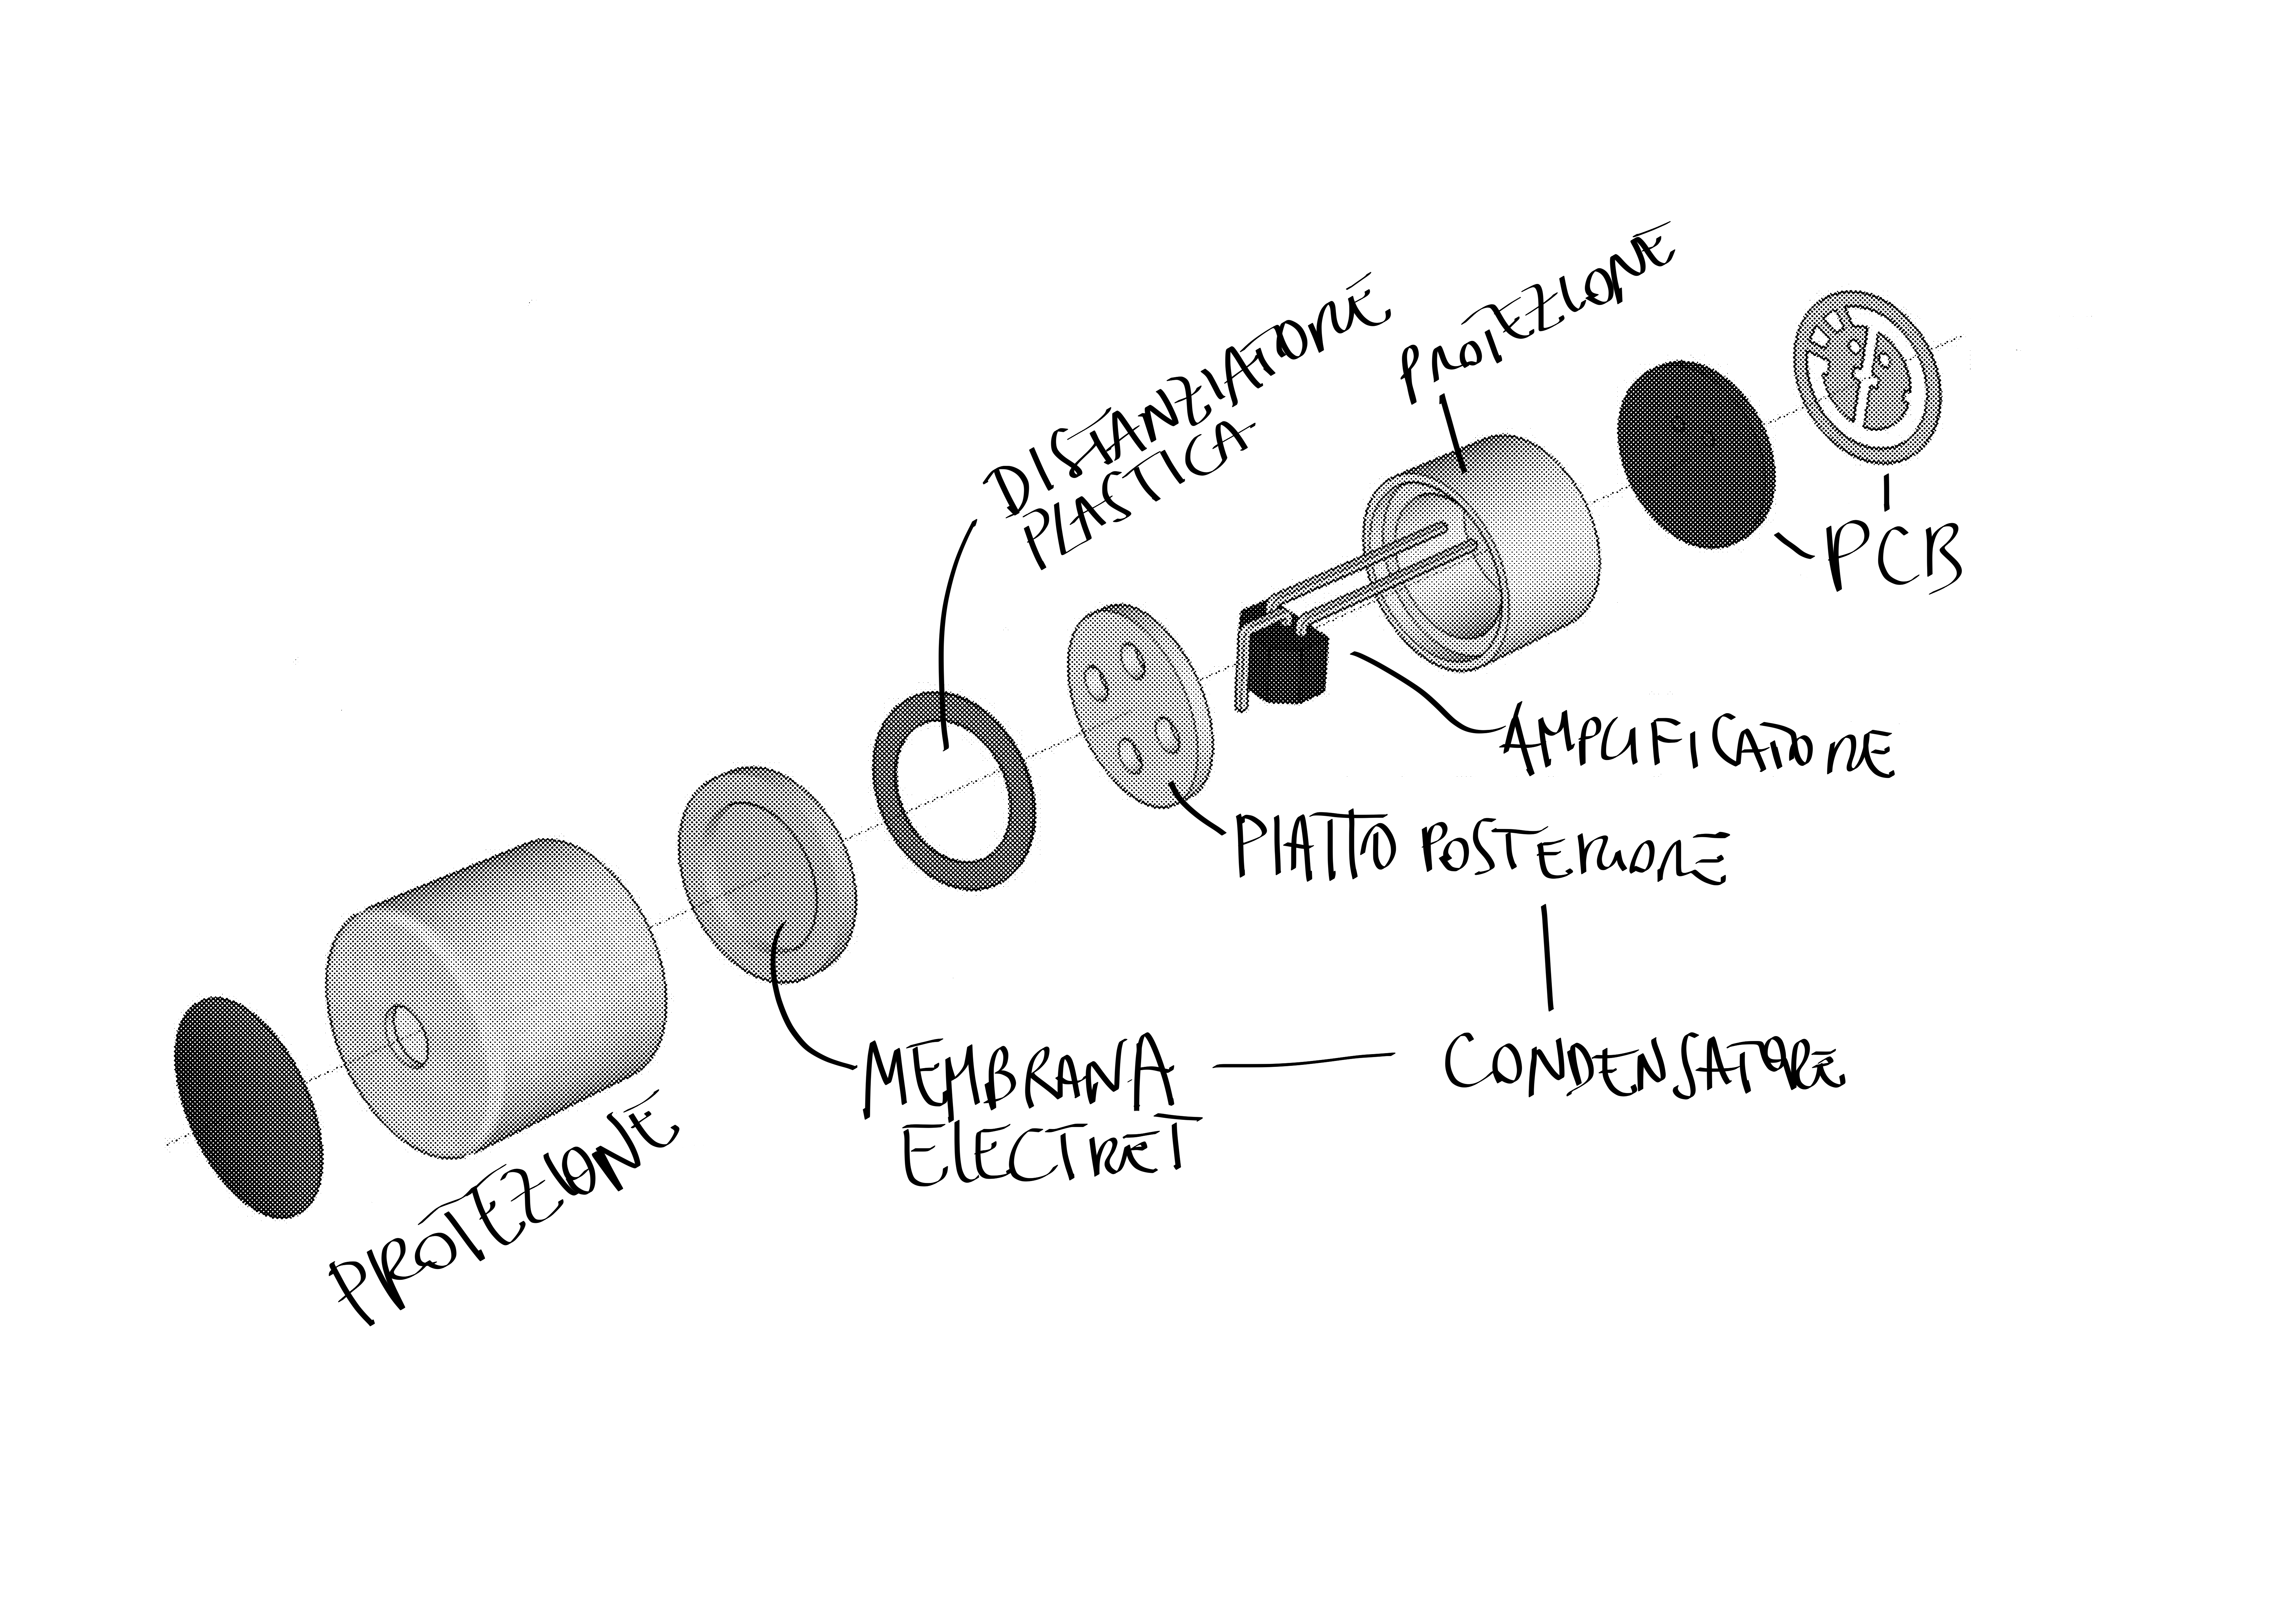
\includegraphics[width=0.99\columnwidth]{CAPITOLI/0200/img/electret.png}
\caption[]{Microfono a condensatore electret.}
\label{mic:electret}
\end{figure}

Il microfono a condensatore di tipologia \emph{electret} è quindi a tutti gli effetti
considerabile una variante nel campo dei microfoni a condensatore (\emph{ECM,
Electret Condenser Microphone}). La particolarità di questi microfoni è che tra
il diaframma e il backplate è inserito un dielettrico di materiale isolante
(electret) il quale ha la caratteristica di essere pre-polarizzato
elettricamente, in modo simile ad un magnete permanente nel campo del magnetismo.
In tal modo, il diaframma non necessita della tensione di polarizzazione,
sebbene questi microfoni siano comunque dotati di un circuito di preamplificazione,
per cui possono essere alimentati da alimentazione fantasma molto bassa o da batteria.
Sebbene questa tecnica sia sorta con l’intento di abbassare i costi, e
quindi sia stata implementata in prodotti economici rivolti più alle registrazioni
amatoriali che a quelle professionali, i progressi effettuati la collocano ormai
quasi alla pari con i migliori microfoni a condensatore. Tra i microfoni electret
i migliori sono da considerarsi quelli dove il dielettrico è solidale con il
backplate, che ne costituisce una delle superfici: essi prendono il nome di
\emph{back-electret}.

% Nella fig. 4 vediamo lo schema in sezione di un microfono electret, e possiamo
% notare come l’esiguità dei componenti lo rendano un dispositivo estremamente
% adatto alla miniaturizzazione, quindi adatto, ad es., ai microfoni a clip.

% \subsubsection{Parametri elettrici}
%
% A chiusura di questa panoramica sull’architettura dei microfoni occorre fornire
% qualche elemento sui parametri elettrici forniti a corredo dei microfoni. Oltre
% alle caratteristiche polari, di cui si parlerà di seguito, i valori più
% significativi per la valutazione di un microfono “sulla carta” sono:
%
% 1) La sensibilità
% 2) Il rumore
% 3) L ’impedenza
% 4) La risposta in frequenza
%
% La sensibilità indica il livello di segnale elettrico che il microfono pu
% fornire a fronte di una determinata pressione acustica sonora. Questo parametro
% ci fornisce un’indicazione utile per determinare quanto il segnale che il
% microfono produce dovrà essere amplificato negli stadi successivi. Così ad es.
% un microfono dinamico può fornire la seguente indicazione di sensibilità:
%
% 2 mV/Pa
%
% ossia 2 millivolt per una pressione acustica sonora di 1 Pascal2. Diamo di seguito,
% indicativamente, una tabella comparativa delle tipologie di microfoni presi in esame:
%
% Il parametro per valutare il rumore introdotto da un microfono è noto come
% “Equivalent Noise Level” (anche “self-noise level”, ossia il rumore inerente
% al microfono), e si riferisce ad un livello di pressione sonora che corrisponde
% al rumore interno del microfono, ossia al suono di livello minimo che è
% possibile registrare con un dato microfono. La scala di misurazione è quella
% del dBSPL , che sarà trattato in altra lezione, ed i metodi di misura sono
% generalmente di due tipi, in base alla curva di pesatura che viene applicata:
% 1) la scala dB(A), complementare delle curve isofoniche di Fletcher-Munson,
% mediante la quale i valori ottimali per i microfoni sono quelli al di sotto di
% 15 dB;
% 2) la scala CCIR 468-1, anche nota come ITU-R 468, che differisce dalla curva
% (A) per una maggiore enfasi nella zona da 5KHz a 8KHz, che fornisce valori
% ottimali al di sotto di 25-30 dB.
%
% In fig. 5 possiamo confrontare le due curve.
%
% L’impedenza del microfono (vedi fig. 6), di cui abbiamo già trattato,
% rappresenta quel valore resistivo che viene “visto” dall’apparecchio collegato
% in successione (preamplificatore, mixer, ecc.).
%
% Come si può osservare in tab. 2, il valore tipico dei microfoni professionali
% è di 200 Ohms, ma con oscillazioni che possono andare da 50 a 600 Ohms.
%
% Risposta in frequenza
%
% Vi sono diversi modi di rappresentare il comportamento di un microfono rispetto
% alle frequenze dei suoni in entrata e rispetto all’angolo d’incidenza degli stessi.
% Uno di questi, la curva di risposta in frequenza, rappresentato in fig. 7, è un
% grafico dove i parametri sono dati dall’ampiezza del suono (sull’asse verticale)
% e dalla sua frequenza (sull’asse orizzontale), e dove i diversi angoli, ch
% rappresentano la quantificazione dello scostamento della provenienza del suono
% rispetto all’asse, sono rappresentati da una famiglia di curve, in cui ad ogni
% curva è associato un valore angolare.
%
%   Curve polari
%
% Il diagramma polare (o curva polare) è invece un grafico a disegno circolare dove i parametri sono dati dall’ampiezza e dall’angolo d’incidenza, mentre le frequenze sono rappresentate da famiglie di curve. In presenza di un’unica curva, si intende che questa è riferita ad una frequenza di 1 KHz.
% Il disegno nella parte sinistra di fig. 8 rappresenta la struttura di un tipico microfono a pressione (pressure microphone) omnidirezionale, mentre nella parte destra è rappresentata la sua curva polare, dove vediamo che la direzionalità del suono inizia ad essere percepita dal microfono a partire da circa 5 KHz in su, mentre le frequenze gravi non sono indicate in quanto assimilabili a quella rilevata a 1 KHz, cioè con attenuazione zero per qualsiasi angolo di provenienza del suono.
%
% Per comprendere il principio di funzionamento di un microfono a pressione dobbiamo immaginare il diaframma di un microfono, sia esso dinamico o a condensatore, come la pelle di un tamburo tesa sopra un contenitore ermeticamente chiuso (backchamber, in figura) Avremo quindi un dispositivo che oscilla in presenza di variazioni di pressione provenienti esclusivamente dall’esterno, essendo la parte interna a pressione costante. Tale trasduttore è per questo motivo chiamato microfono a pressione, ed essendo le variazioni di pressione indipendenti dall’angolo di arrivo delle stesse, la caratteristica polare fa di questo dispositivo un microfono omnidirezionale.
% La possibilità di reagire in modo uniforme ad ogni direzione di provenienza del suono è in realtà teorica, come si può perfettamente osservare guardando la sua curva polare, in quanto per il principio della diffrazione acustica le frequenze della gamma alta tenderanno ad attenuarsi al crescere dell’angolo di incidenza a partire dall’asse del microfono, mentre tenderanno ad elevarsi al diminuire dello stesso angolo di incidenza, ossia man mano che l’angolo di arrivo va a coincidere con l’asse. Il fenomeno è dovuto
%
% alla presenza fisica del microfono stesso nel campo sonoro che interferisce con la propagazione delle onde sonore. Un microfono che, per la sua costruzione fisica, dovuta essenzialmente al ridotto diametro del diaframma, sia esente da questo fenomeno è detto microfono a campo libero (free-field microphone). Un microfono a pressione può lavorare come microfono a campo libero nel momento in cui gli venga applicata una correzione acustica e/o una equalizzazione (free-field correction) che rendano il suo comportamento lineare alle frequenze alte.
% La caratteristica di esaltazione delle frequenze alte in asse è stata, nel corso della storia, sfruttata al fine di ottenere la linearità che si perde naturalmente con la distanza per via della densità dell’aria, che tende a penalizzare proprio le frequenze alte. Nella fig. 9 vediamo un esempio di applicazione di sfruttamento del fenomeno col microfono Neumann M50, in cui il diaframma è incastonato in una forma sferica, con l’intento di interferire maggiormente col campo libero. Nella parte destra vediamo la sua curva caratteristica, che lo hanno reso una scelta preferita nelle riprese panoramiche di orchestre.
%
% Nella fig. 10 abbiamo la rappresentazione di una curva sensibilmente differente dalla prima, in quanto vediamo che l’attenuazione del segnale ha il suo punto massimo a 180° (alle spalle del microfono), ed è già significativa (circa 12 dB) a 500 Hz. Tale curva polare descrive il comportamento di un microfono direttivo noto come microfono cardioide. Il termine
%
%
% “cardioide” deriva dalla forma a “cuore rovesciato” che tende ad assumere la curva polare.
%
% E’ importante evidenziare che la direzionalità del microfono è ottenuta mediante l’apertura, alle spalle del diaframma, di fessure la cui funzione è di far pervenire parte del suono sul retro del diaframma, generando un’opposizione di fase in grado di agire sui suoni laterali e posteriori, come illustrato in fig. 11.
% In conseguenza del fatto che il diaframma è aperto nella zona retrostante, il microfono è detto microfono a gradiente di pressione (pressure gradient microphone), in quanto la sua risposta è generata dal rapporto della pressione frontale con quella posteriore.
% Dal momento che il percorso che compie il suono in entrata alle fessure laterali è un percorso finito, mentre i suoni possono avere frequenze diverse, l’opposizione di fase è “accordata” sulle frequenze medio-alte per evidenziare la direttività. A causa di ciò esiste un effetto collaterale derivante da questa tecnica, consistente nel fatto che, nel momento in cui il microfono direzionale è installato molto vicino alla fonte sonora, si genera un’esaltazione innaturale delle frequenze gravi, dovuta proprio alla presenza delle aperture laterali. Questo effetto, che può anche essere adoperato in modo appropriato per ottenere un suono particolarmente “caldo” ad es. nella voce, prende il nome di effetto di prossimità (proximity effect).
%
% Aumentando la lunghezza della zona del corpo microfono aperta da fessure, come nel microfono di fig. 12, si aumenta la caratteristica direzionale del microfono, la cui curva prende il nome di supercardioide. A causa della ridotta efficacia dell’accordatura laterale per i suoni a 180°, compare nella curva un lobo posteriore che sposta il punto di attenuazione massima dai 180° della curva cardioide a circa 135° (225° nel terzo quadrante). Nei microfoni a curva ipercardioide è ulteriormente ristretta l’angolazione frontale, mentre viene accentuata la caratteristica del lobo posteriore, rendendoli una soluzione intermedia tra la curva supercardioide e la curva a figura-8 di cui parleremo più avanti. Il punto di attenuazione massima è ora intorno a 110° (250° nel terzo quadrante), come illustrato in fig. 13.
%
% Tra i microfoni a gradiente di pressione, esistono infatti dei microfoni, detti a figura 8, la cui curva polare, illustrata in figura 14, presenta una simmetria avanti/dietro, dove i punti di attenuazione massima si vanno a situare a 90° e 270°. Tali microfoni hanno uguale sensibilità per i suoni provenienti dal fronte e dal retro, mentre tendono ad annullare i suoni di provenienza laterale. I microfoni a nastro di cui abbiamo parlato sono caratterizzati da tale curva.
%
% Per chiudere la panoramica delle curve polari è opportuno notare come esse possano venire espresse da funzioni trigonometriche, in modo da descrivere il valore punto per punto della curva partendo dall’angolo di incidenza del suono, come evidenziato in fig. 15.
%
% A completamento della panoramica sulle tecniche costruttive impiegate per ottenere la possibilità di variare la direzionalità del microfono è importante accennare ai microfoni a condensatore che si avvalgono di un doppio diaframma installato al loro interno. Nella fig. 16 notiamo come due diaframmi sono montati “spalla a spalla” (back-to back) con in mezzo il backplate. La combinazione di intensità e di fase delle due membrane può fornire una gamma di caratteristiche polari diverse, dalla omnidirezionale alla figura 8, fino alla cardioide e all’ipercardioide. Tale configurazione è nota anche come “Braunmühl/Weber” dai nomi dei suoi inventori (1937), e si avvale tipicamente di diaframmi a largo diametro, a differenza dei microfoni a pressione che per avere
% maggiore omnidirezionalità devono essere forniti di un diaframma di piccolo diametro.
%
% Per particolari situazioni in cui è richiesta poca intrusività visiva del dispositivo di ripresa sono adoperati dei microfoni, detti pressure zone microphones o anche boundary microphones, illustrati in fig. 17, la cui architettura consiste in una capsula omnidirezionale montata molto vicino ad una piastra piana, la quale a sua volta va utilizzata a
% contatto con una superficie (pavimento, muro, tavolo, ecc.). Il principio consiste nel fatto che, diversamente da quel che accade in un microfono tradizionale montato, ad es., su un’asta, il suono diretto dallo strumento non è degradato, per effetto di comb-filter, dalle riflessioni dell’ambiente circostante, ma, grazie a questo disegno, le onde sonore arrivano tutte egualmente riflesse dalla piastra verso la capsula, e quindi perfettamente in fase. In pratica la superficie d’appoggio agisce da barriera del suono, e il microfono è così in grado di captare il suono senza cancellazioni di fase dovute a riflessioni. La curva polare che tale microfono genera, in virtù del suo posizionamento su di una superficie, è così una curva emisferica, cioè una curva semi-omnidirezionale (half- omnidirectional) che si irradia “al di sopra” del microfono.
%
%
% Esistono infine dei microfoni, detti “parabolici”, schematizzati in fig. 18, che si avvalgono della proprietà acustica di una superficie paraboloide di concentrare per riflessione le onde sonore in un unico punto (fuoco della parabola) consentendo a dei normali microfoni di assumere delle caratteristiche di spiccata direttività, di molto superiore a quella fornita dai microfoni ipercardioidi. L ’utilizzo di tali microfoni è chiaramente limitato ad alcuni ambiti, come la ripresa a bordo campo di eventi sportivi, la cattura a grande distanza di suoni del mondo animale per scopi scientifici e documentari naturalistici, e le intercettazioni ambientali.
%
% Naturalmente, la risposta in frequenza di un tale dispositivo non potrà mai essere a banda piena, ma presenterà un’inevitabile carenza sulle basse frequenze, in quanto la parabola sarà in grado di
% riflettere solamente i suoni con lunghezza d’onda sensibilmente inferiore al valore del suo diametro.
% I vantaggi che può dare un tale dispositivo si possono verificare nella fig. 19: il microfono è tanto più efficiente quanto più largo è il diametro della parabola, fornendo un guadagno sul segnale che può arrivare a 30 dB a 8.000 Hz.

%%%%%%%%%%%%%%%%%%%%%%%%%%%%%%%%%%%%%%%%%%%%%%%%%%%%%%%%%%%%%%%%%%%% SUBSECTION
%%%%%%%%%%%%%%%%%%%%%%%%%%%%%%%%%%%%%%%%%%%%%%%%%%%%%%%%%%%%%%%%%%%%%%%%%%%%%%%%
\subsection{Sul concetto di \emph{Figura Polare}}
\label{sec:polarplot}

La figura polare di un microfono è la rappresentazione grafica su di un piano,
nel sistema di coordinate polari, della sensibilità in funzione dell'angolo di
incidenza del suono sulla membrana. Questo tipo di figura polare si presenta
come una linea curva chiusa (o insieme di più linee di questo tipo, tipicamente
associate alle ampiezze polari in risposta a diverse frequenze). In presenza di
un’unica curva la si intende riferita ad una frequenza di $1KHz$ in rappresentazione
di un valore generico di intensità di risposta del microfono stesso,
e come tale fornisce una rapida indicazione visiva di come l'intensità di
risposta sia geometricamente distribuita intorno
al microfono stesso.

\begin{figure}[h]
\centering
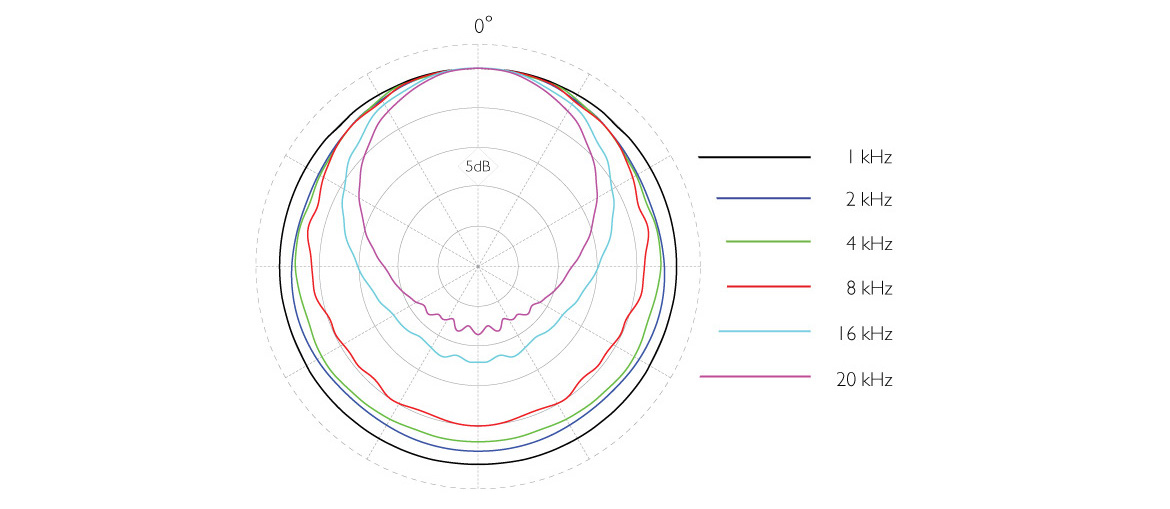
\includegraphics[width=0.99\columnwidth]{CAPITOLI/0300/IMG/4006A-ddicate-4006A-Omni-Microphone-polar-pattern.jpg}
\caption[]{Risposta polare in frequenza del microfono \emph{DPA 4006A}.}% \url{https://www.dpamicrophones.com/pencil/4006-omnidirectional-microphone}.}
\label{pol:dpa4006}
\end{figure}

\begin{figure}[t]
\centering
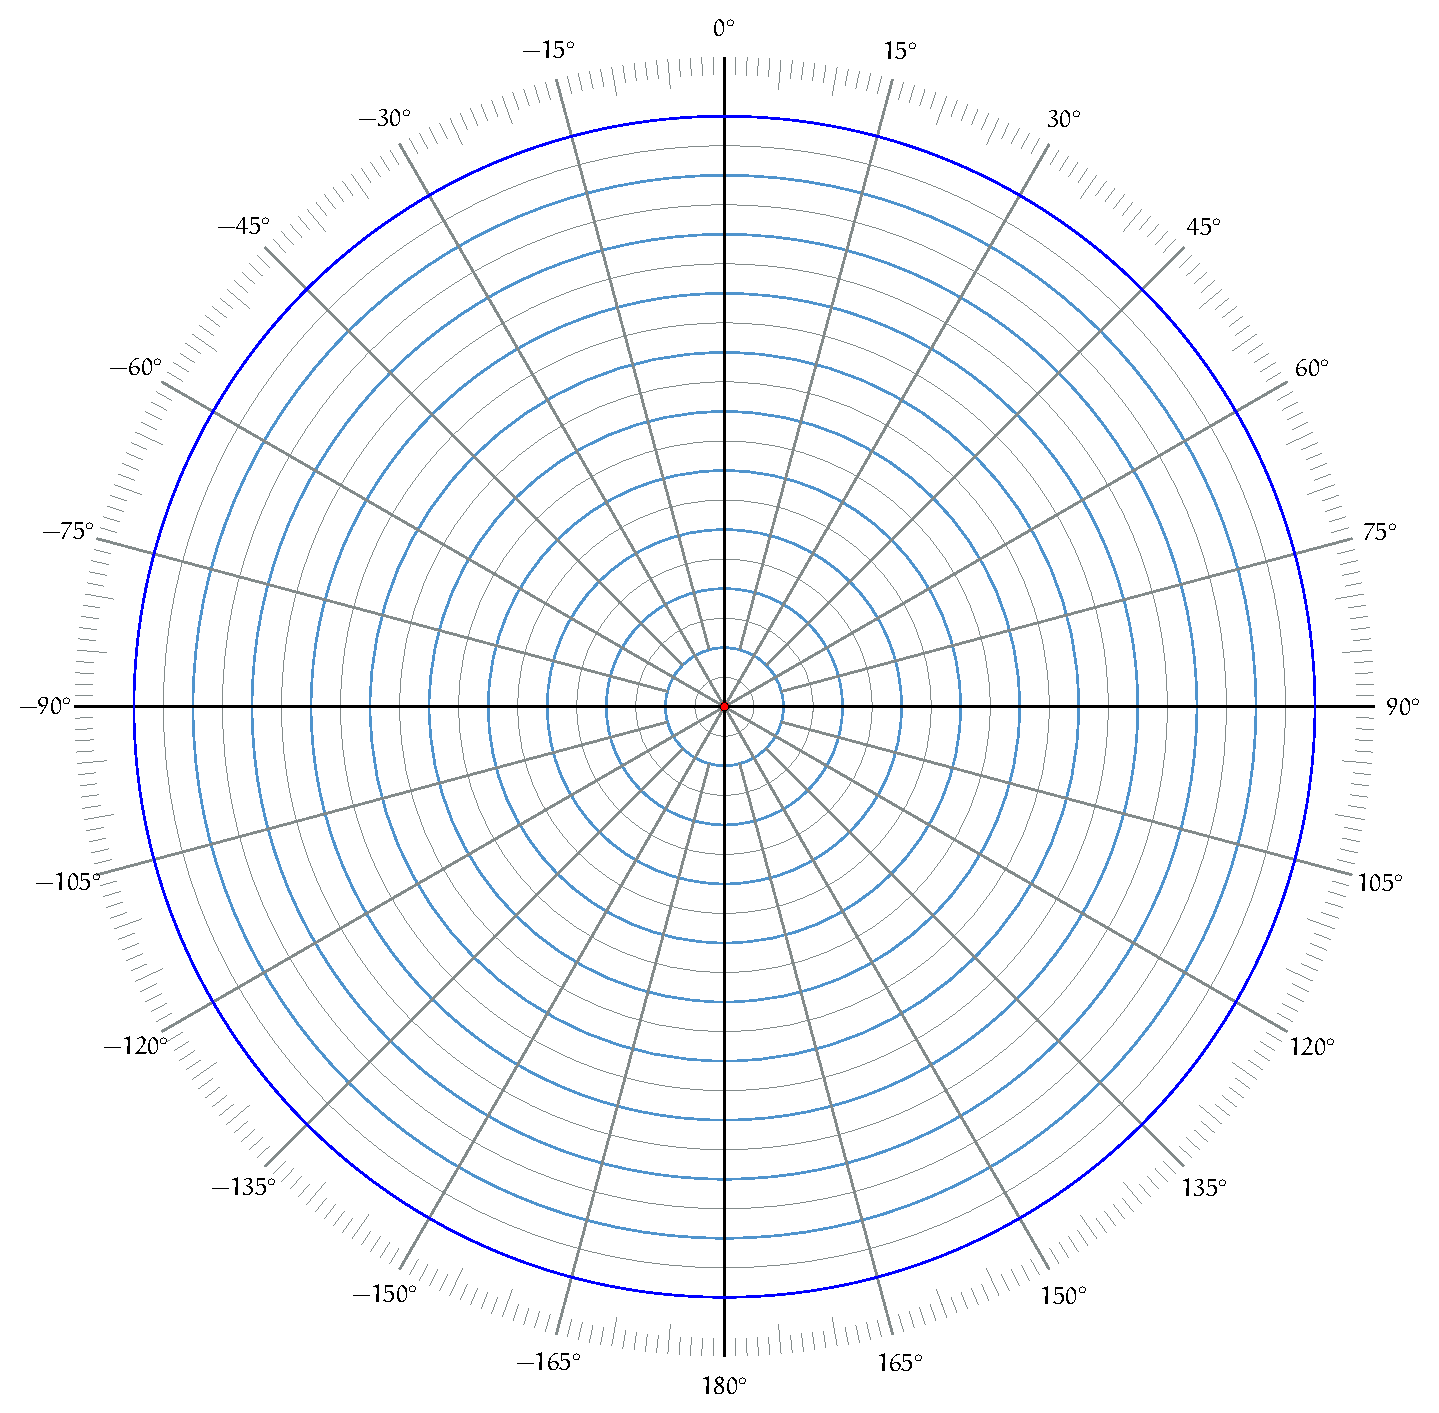
\includegraphics[width=0.99\columnwidth]{microphone-polar-patterns/omni}
\caption[]{Rappresentazione ideale del microfono a pressione mediante la sua
equazione polare: $ndp = 1(x)$ (non-directional pressure). La figura polare
descrive una risposta in fase lineare per ogni angolo di inncidenza.}
\label{polar:omni}
\end{figure}

In un sistema polare ciascun punto è
determinato da una distanza, da un punto di riferimento, ed un angolo, da una
direzione di riferimento. Nel caso di una figura polare di un microfono, il
punto di riferimento è l'origine, il centro del piano e la direzione di
riferimento è il fronte, ovvero l'asse di puntamento frontale del microfono. Per
questa ragione la figura polare del microfonico presenta l'angolo zero
nel nord del piano, si muove angolarmente verso sinistra per angoli
negativi e verso destra per angoli positivi. Il movimento angolare, denominato
\emph{azimuth} è espresso in radianti $(\pi,-\pi)$ ed una eventuale indicazione in
gradi può essere connvertita in radianti mediante l'equazione $deg = \pi/180$,
con valori negativi a sinistra e positivi a destra.

Un segnale nella sua oscillazione espressa nella variazione di ampiezza
attorno allo zero potrebbe essere derivato da qualsiasi tipo di microfono senza
un significato particolare. Potrebbe essere generato elettricamente da un
microfono con modello polare particolare o generato sinteticamente secondo equazioni polari, senza
alcuna rilevanza specifica in termini di descrizione dell'andamento di ampiezza.
La provenienza polare, la forma che assume la fase del segnale, diventa rilevante nel confronto tra segnali.

La figura polare ideale di un microfono che non trasferisce informazioni relative
alle variazioni dell'angolo di incidenza del suono è definita dall'equazione:

\begin{equation}
ndp = 1(x)
\label{eq:omni}
\end{equation}

Un microfono di questo tipo descrive esclusivamente variazioni di ampiezza
derivate della variazione di pressione dell'aria, motivo per cui è definito
microfono a pressione, e risponde alla figura polare \emph{non-direzionale}, anche se
nel mercato dei microfoni si è imposto con il nome \emph{omni-direzionale}.

La membrana di un microfono di questo tipo è stesa, come la pelle di un tamburo a fusto chiuso.
Il dispositivo oscilla in presenza di variazioni di pressione provenienti esclusivamente dall’esterno,
essendo la parte interna a pressione costante. Idealmente le variazioni di pressione sono indipendenti
dall’angolo di incidenza sulla membrana. Nella realtà fisica fisica la membrana
è sottoposta a fenomeni di diffrazione acustica che ne modificano la risposta polare in frequenza.
Le frequenze acute tendono a descrivere variazioni di sensibilità al variare
dell’angolo di incidenza del suono in relazione al fronte microfonico.
I fenomeni di diffrazione acustica avvengono in relazione alla presenza fisica
del microfono stesso nel campo sonoro che interferisce con la propagazione delle
onde sonore ad alta frequenza, ostacolandole.

La figura \ref{pol:dpa4006} rappresenta la curva polare di un ottimo microfono
omni-direzionale. Si può osservare che la caratteristica non-direzionalità di
percezione del suono è reale solo per un range di frequenze, mentre il microfono
inizia ad ad avere un carattere direzionale da circa per le frequenze acute.
Le frequenze gravi sotto a $1KHz$ non sono descritte singolarmente perché
assimilabili alla frequenza di riferimento di $1KHz$. Lo stesso microfono può essere
equipaggiato da correttori acustici per la ripresa sonora in campo libero. Lo
scopo di questi correttori acustici è proprio quello di avvicinare la resa del
microfono alla figura polare ideale non-direzionale, come mostrato in figura \ref{pol:dpa4006nose}.

\begin{figure}[h]
\centering
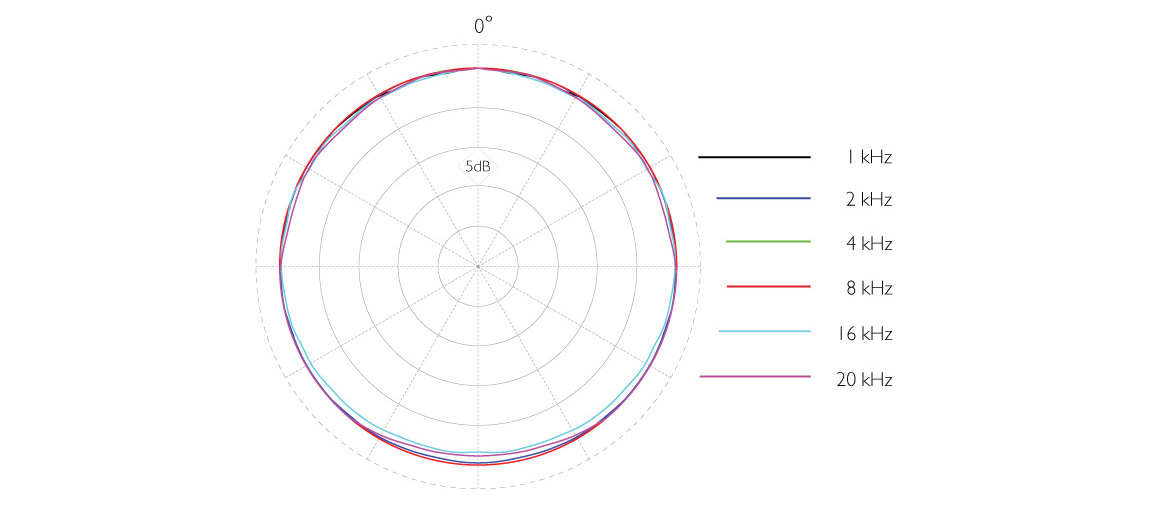
\includegraphics[width=0.99\columnwidth]{CAPITOLI/0300/IMG/4006A-ddicate-4006A-Omni-Microphone-polar-pattern-nose-cone-veritical.jpg}
\caption[]{Risposta polare in frequenza del microfono \emph{DPA 4006A} con \emph{Nose Cone AU0777}, microfono con posizionamento verticale.}% \url{https://www.dpamicrophones.com/pencil/4006-omnidirectional-microphone}.}
\label{pol:dpa4006nose}
\end{figure}

\begin{figure}[t]
\centering
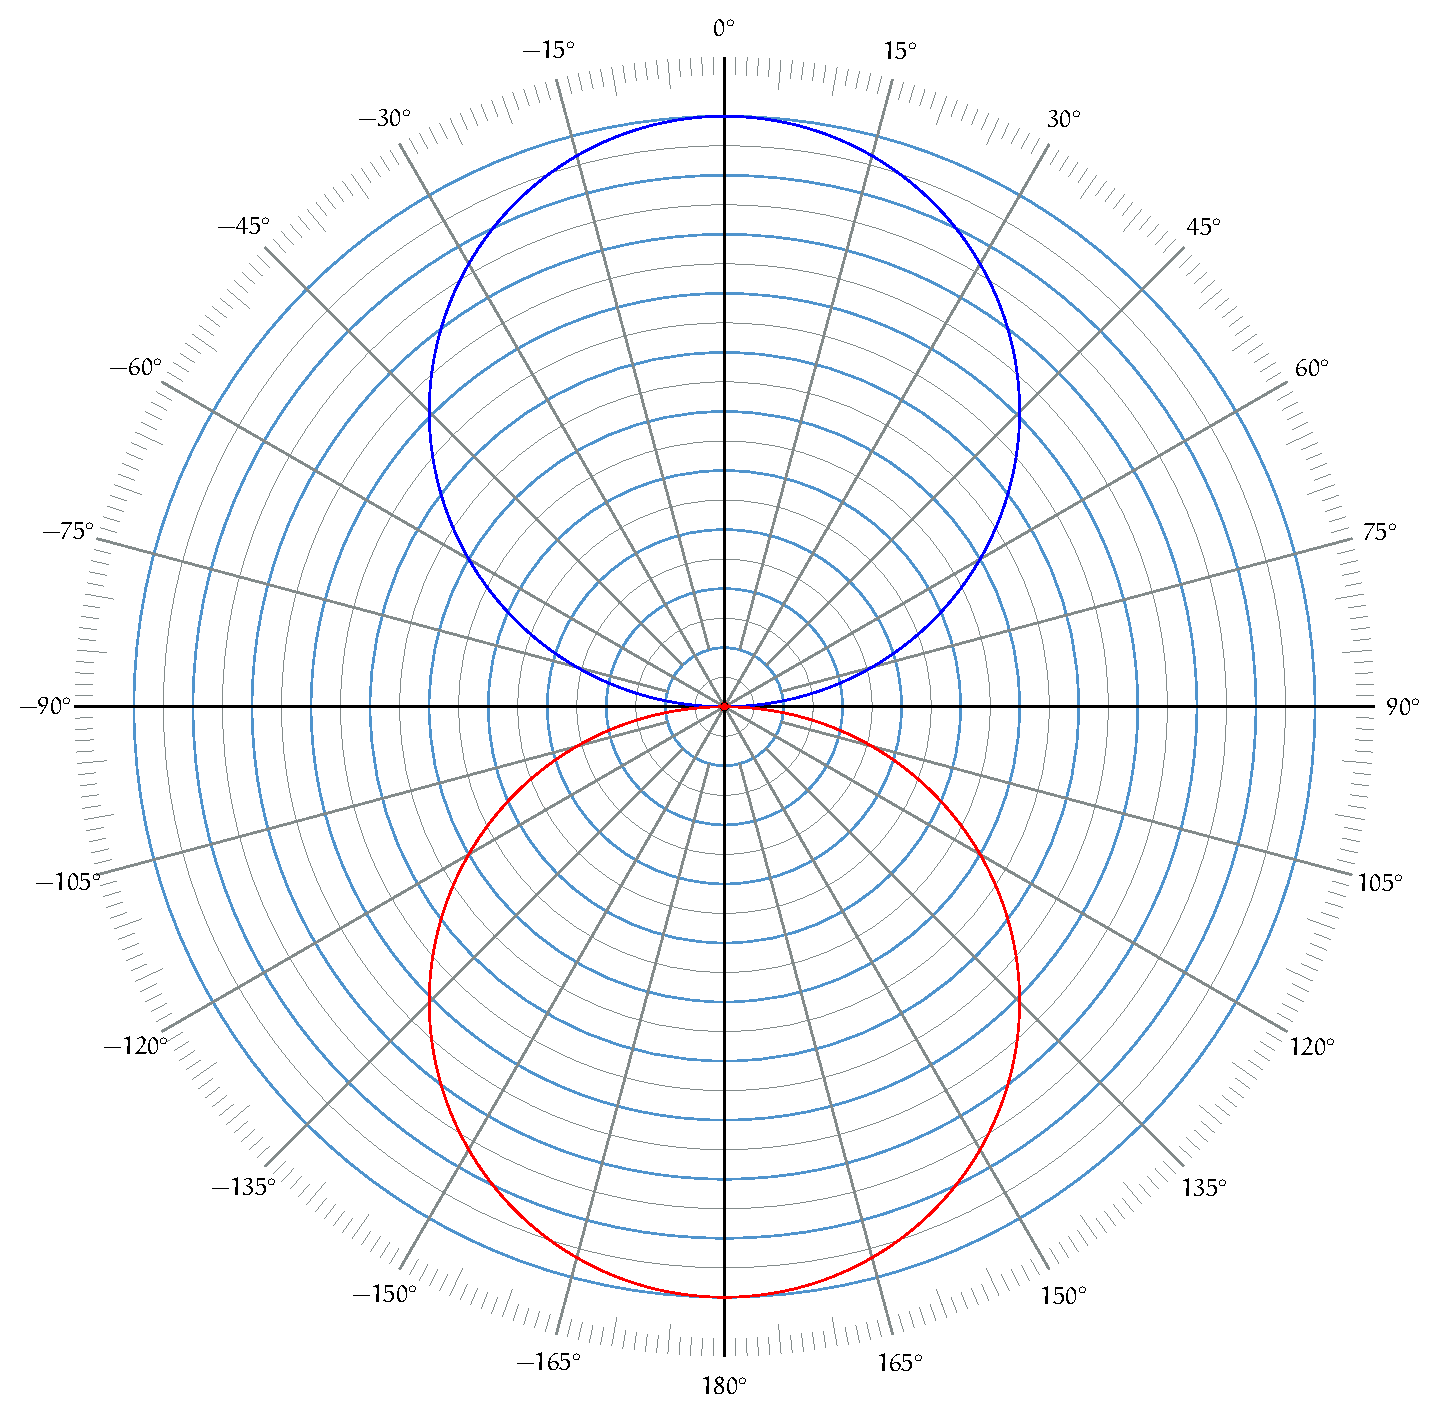
\includegraphics[width=0.99\columnwidth]{microphone-polar-patterns/fig8}
\caption[]{Rappresentazione ideale del microfono bidirezionale a gradiente di
pressione mediante la sua equazione polare: $bpg = x\cos\theta$
(\emph{bidirectional pressure gradient}). La figura polare descrive una risposta
in fase bipolare, positiva per angoli di incidenza frontali ($[(0,\pi/2),(0-\pi/2)]$),
negativa per angoli di incidenza posteriori ($[(-\pi,\pi/2),(-\pi,\pi/2)]$)}
\label{polar:fig8}
\end{figure}

\begin{figure}[t]
\centering
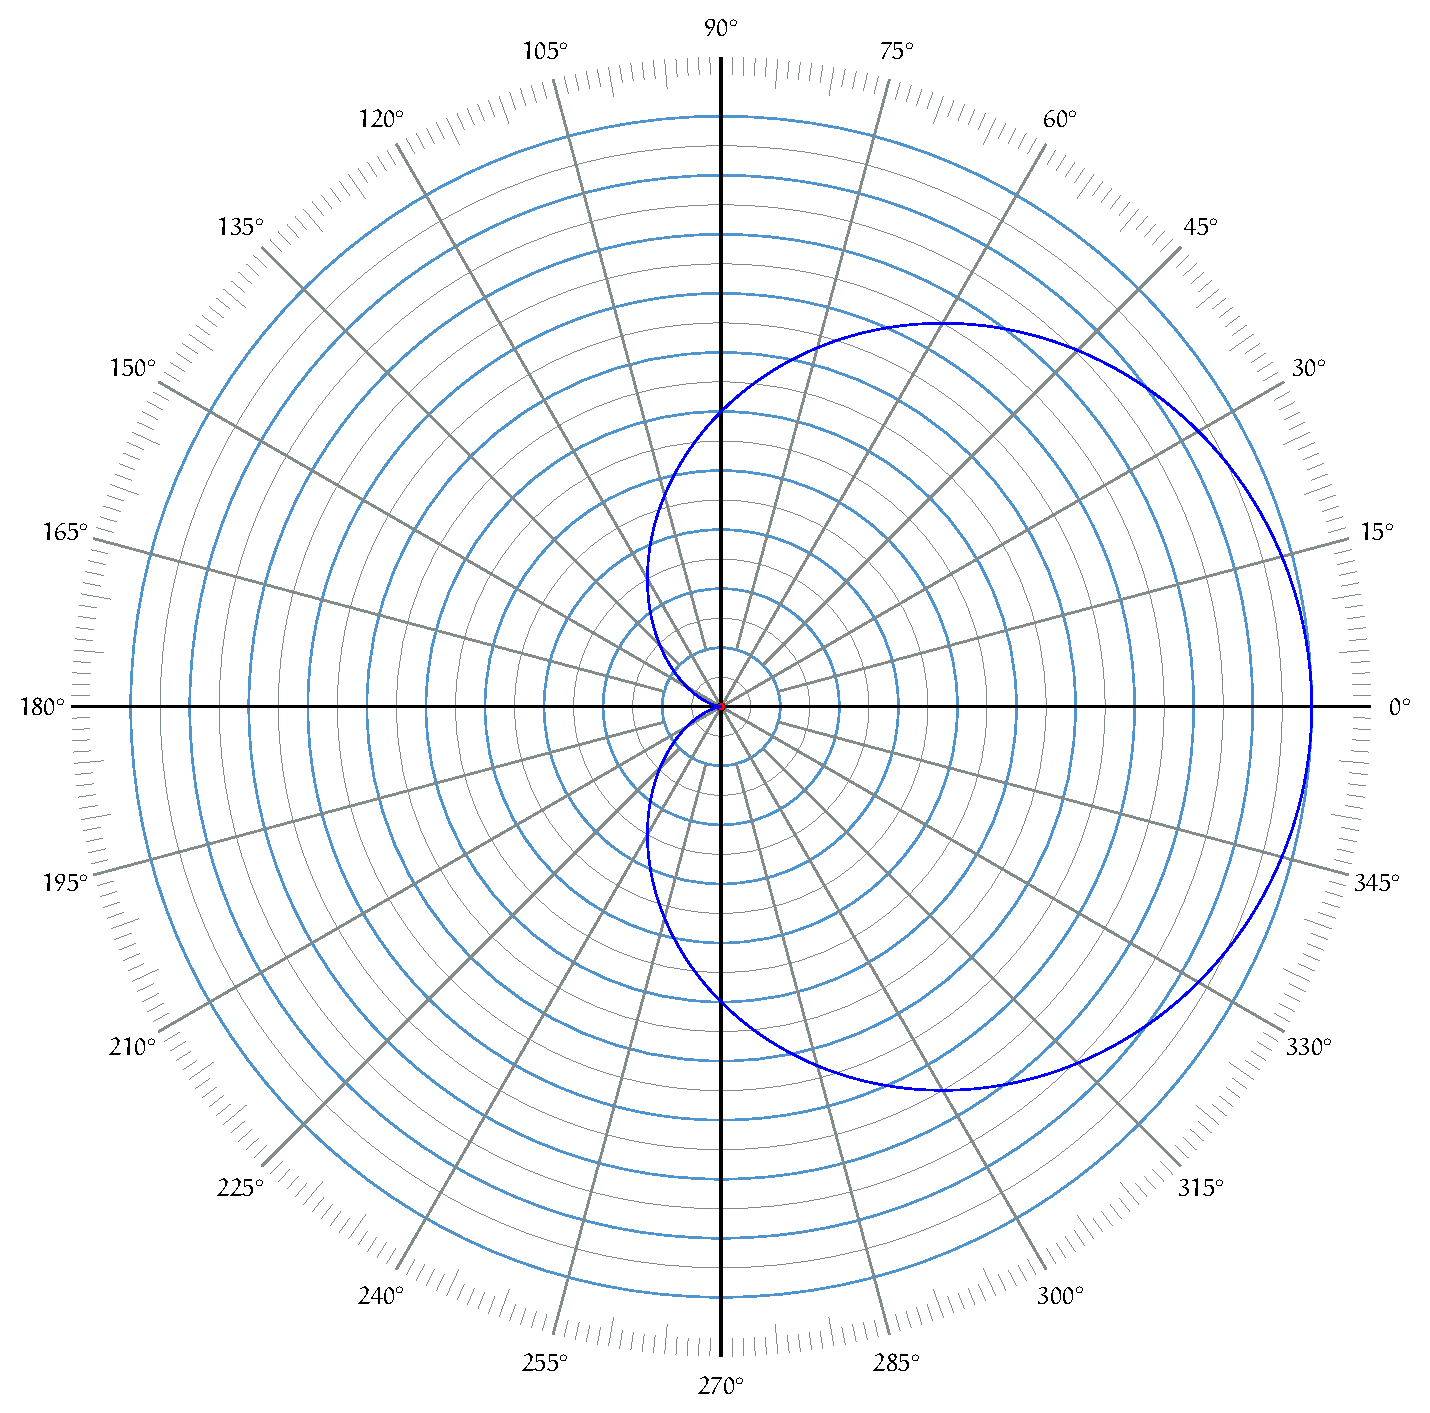
\includegraphics[width=0.99\columnwidth]{microphone-polar-patterns/cardioid}
\caption[]{Rappresentazione ideale del microfono direzionale cardioide a gradiente
di pressione mediante la sua equazione polare: $cpg = 0.5(x) + 0.5(x\cos\theta)$
(\emph{cardioid pressure gradient}). La figura polare descrive una risposta in
fase positiva non lineare per diversi angoli di inncidenza.}
\label{polar:cardioid}
\end{figure}

I microfoni che per cratteristiche costruttive presentano principi di direzionalità
vengono definiti \emph{microfoni a gradiente di pressione} in quanto la variazione
di pressione dell'aria è percepita in maniera diversa per angoli d'incidenza diversi.
Tra questi, il microfono bidirezionale denominato microfono a \emph{figura-8},
presenta una figura polare simmetrica fronte-retro, con punti di attenuazione
massima a $\pm90°$. Tali microfoni hanno uguale sensibilità per i suoni
provenienti dal fronte e dal retro, mentre tendono ad annullare i suoni di
provenienza laterale. La doppia direzionalità caratterizza una doppia polarità
in quanto i segnali generati da angoli di incidenza posteriori sono caratterizzati da
una fase negativa.

\begin{equation}
bpg = x\cos\theta
\label{eq:fig8}
\end{equation}

La prima differenza rilevante tra un'equazione del modello polare non
direzionale (\ref{eq:omni}) e una direzionale (\ref{eq:fig8}) è la
presenza del coefficiente angolare. L'angolo \emph{theta} nell'equazione
(\ref{eq:fig8}) descrive la direzione polare di puntamento del microfono bidirezionale
espressa in radianti che, nel caso specifico, corrisponde a zero radianti. Il valore di
$x$ esprime la variazione d'ampiezza del segnale relativo alla variazione di pressione.

In termini ideali la somma tra figure polari produce figure risultanti aventi caratteri
di entrambe le figure originarie. In questo modo, sommando pari quantità di componenti
non-direzionale e bipolare, si ottiene una figura polare intermedia che prende il
nome di figura cardioide.

\begin{equation}
cpg = 0.5(x) + 0.5(x\cos\theta)
\label{eq:cardioid}
\end{equation}

Il microfono cardioide appartiene, come il microfono bidirezionale, alla tipologia
gradiente di pressione (\emph{cpg}), in quanto la produzione del segnale elettrico è condizionata
dall'angolo di incidenza.

La figura polare cardioide presenta la sola polarità positiva, una spiccata
sensibilità frontale ed una progressiva riduzione di sensibilità al variare dell'angolo
di incidennza.

Cardioidi e altre figure polari comuni del primo ordine, come anche ogni
sfumatura di forma tra di loro, sono prodotte con diversi coefficienti di peso
tra la pressione non-direzionale e gradiente di pressione bidirezionale,
come in tabella \ref{tab:polarcoef}. Ogni figura direzionale prodotta può avere
un proprio angolo di punatamento intorno a $2\pi$ radianti.

\vfill\null

\clearpage

\begin{table}[ht]
%\scriptsize
\caption[]{Coefficienti di pressione \emph{non-direzionale} e gradiente di pressione
\emph{bidirezionale} per la descrizione dei modelli polari intermedi, del primo ordine.
Dove $x$ è la variazione d'ampiezza del segnale relativa alla pressione in
ingresso e $\theta$ l'angolo di incidenza}
\begin{center}
\begin{tabular}{rrcll}
\textbf{Polar Pattern} & \textbf{NDP} & : & \textbf{BPG} &\\
\hline
non-direzionale & $1(x)$       &     &                      &
 \multirow{4}{*}{\begin{minipage}{.25\textwidth}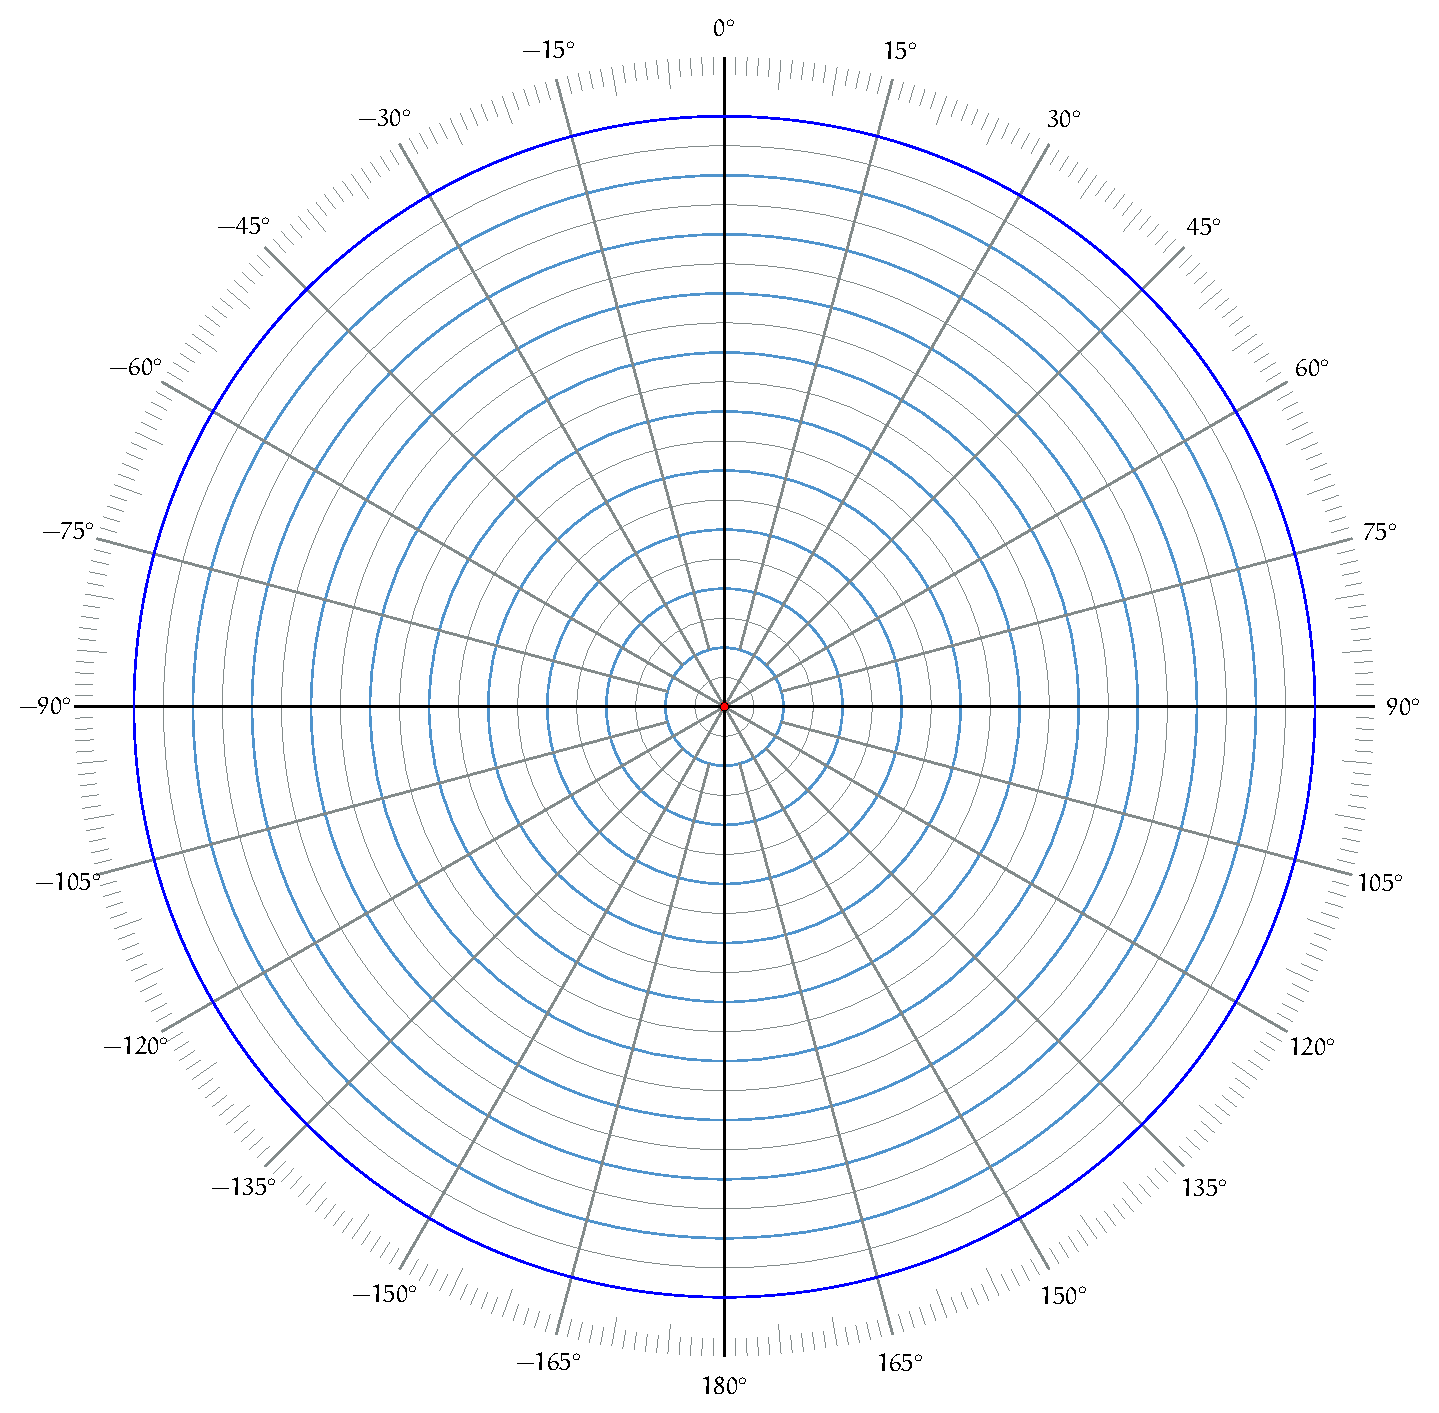
\includegraphics[width=\linewidth]{microphone-polar-patterns/omni}\end{minipage}} \\
                & $1$          & $+$ & $0$                  & \\
                & $0dB$        & $+$ & $-\infty$         & \\ %20*log10(g)
& \\
\hline
subcardioide    & $0.75(x)$    & $+$ & $0.25(x\cos\theta)$  &
 \multirow{4}{*}{\begin{minipage}{.25\textwidth}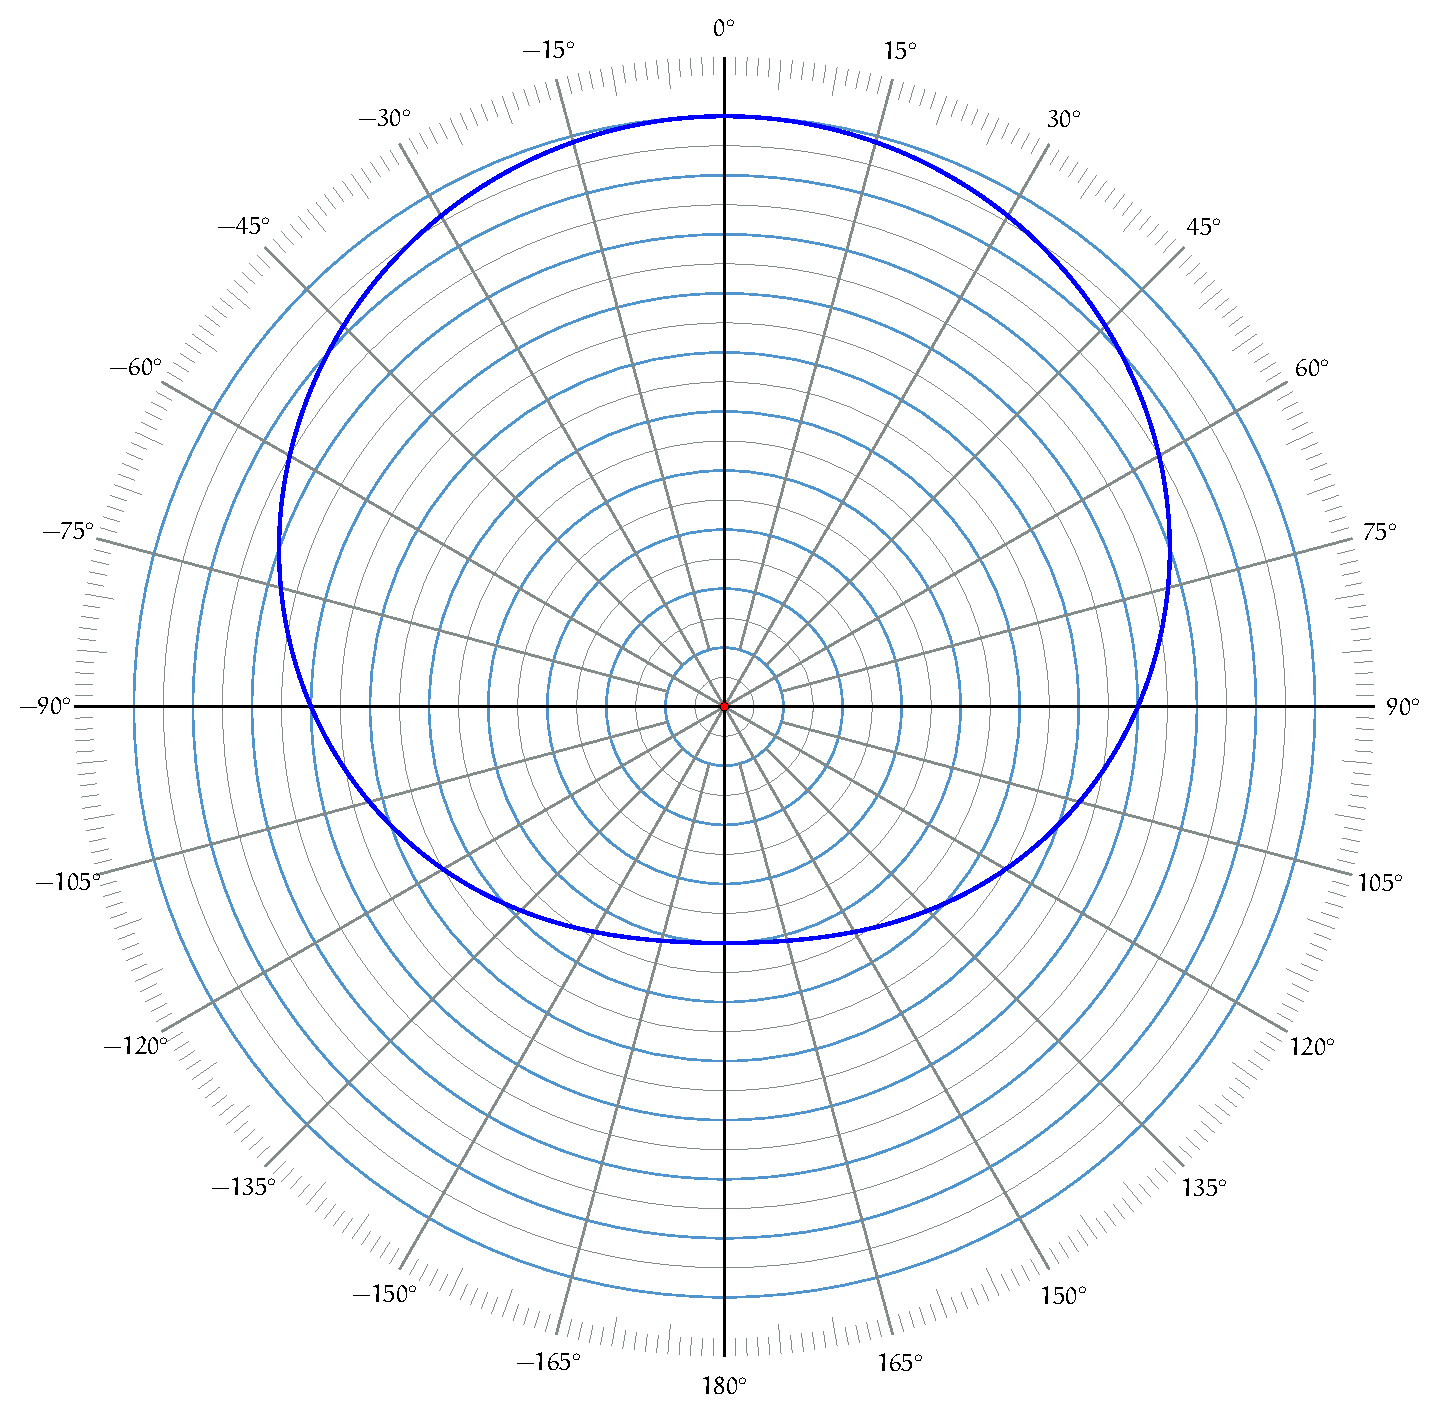
\includegraphics[width=\linewidth]{microphone-polar-patterns/subcardioid}\end{minipage}} \\
                & $0.75$       & $+$ & $0.25$               & \\
                & $-2.75dB$    & $+$ & $-12.05dB$           & \\
& \\
\hline
cardioide       & $0.5(x)$     & $+$ & $0.5(x\cos\theta)$   &
 \multirow{4}{*}{\begin{minipage}{.25\textwidth}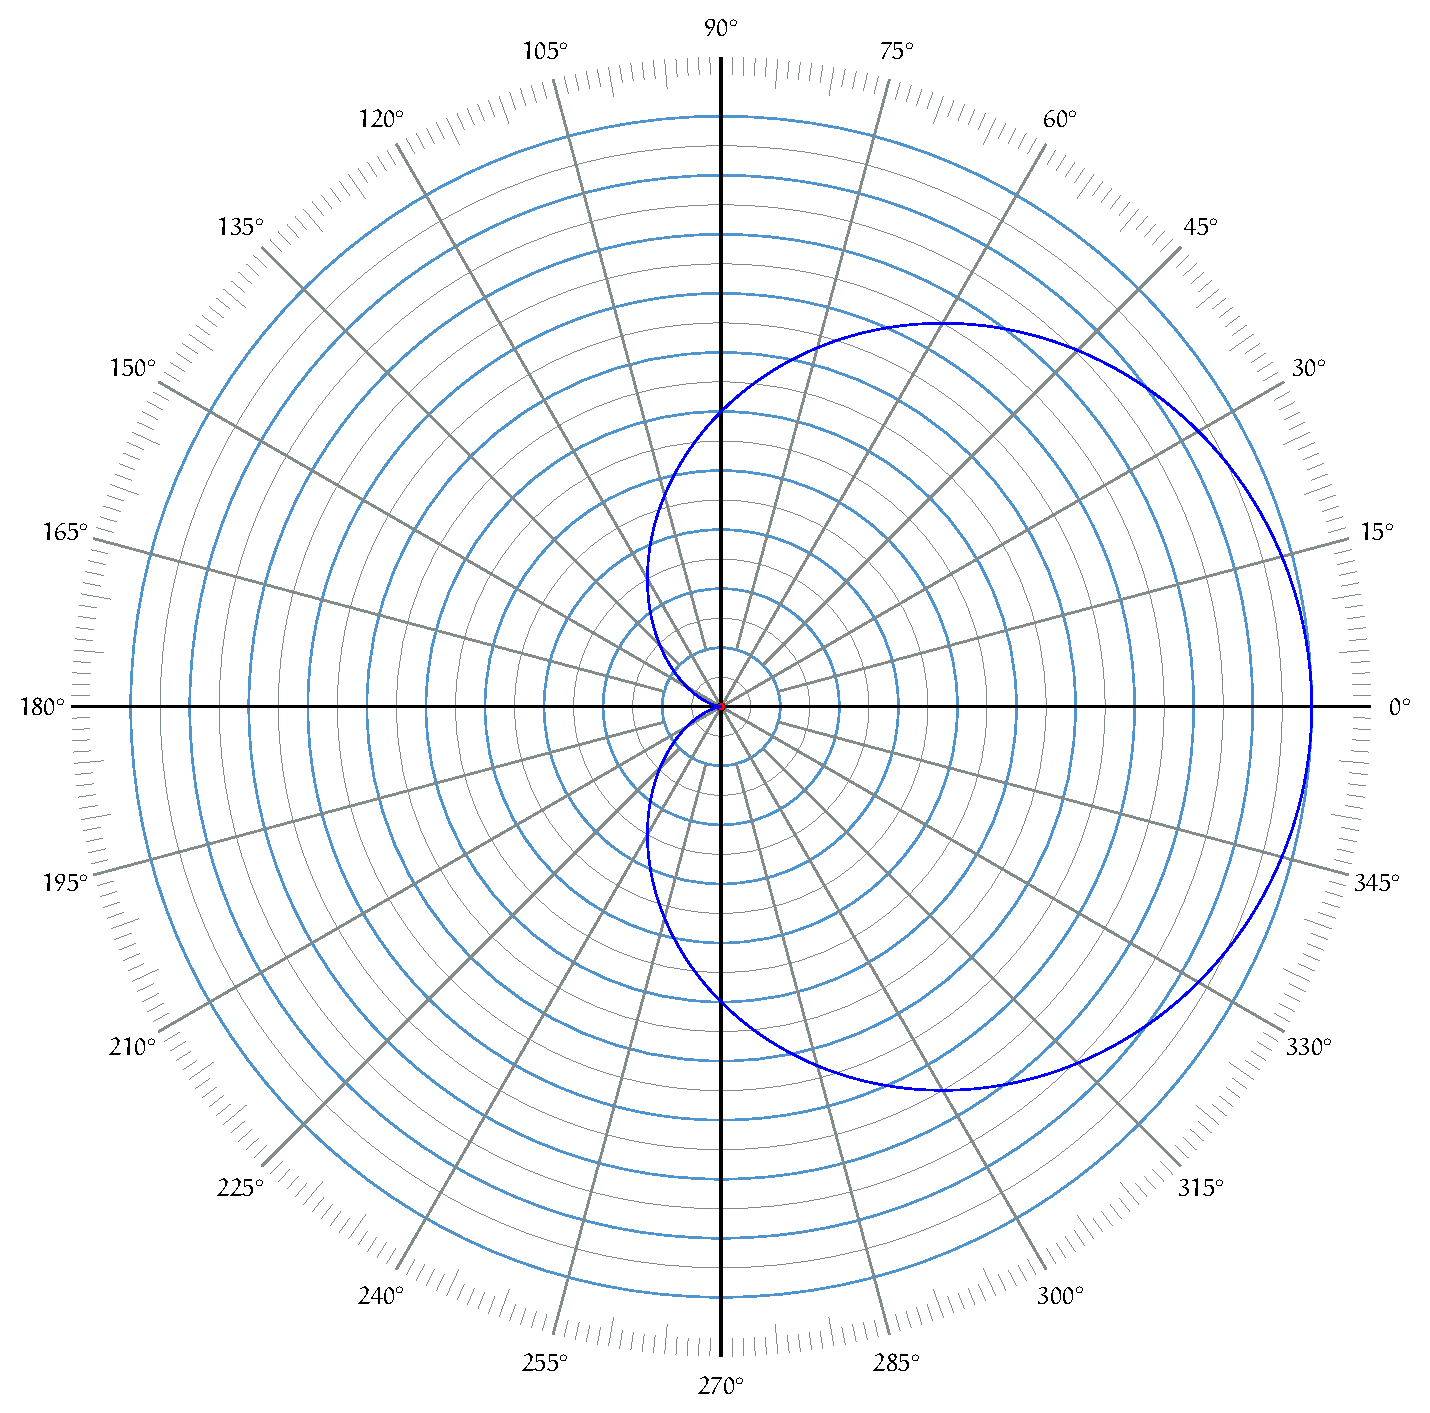
\includegraphics[width=\linewidth]{microphone-polar-patterns/cardioid}\end{minipage}} \\
                & $0.5$        & $+$ & $0.5$                & \\
                & $-6.02dB$    & $+$ & $-6.02dB$            & \\ %20*log10(g)
& \\
\hline
supercardioide  & $0.37(x)$    & $+$ & $0.63(x\cos\theta)$  &
 \multirow{4}{*}{\begin{minipage}{.25\textwidth}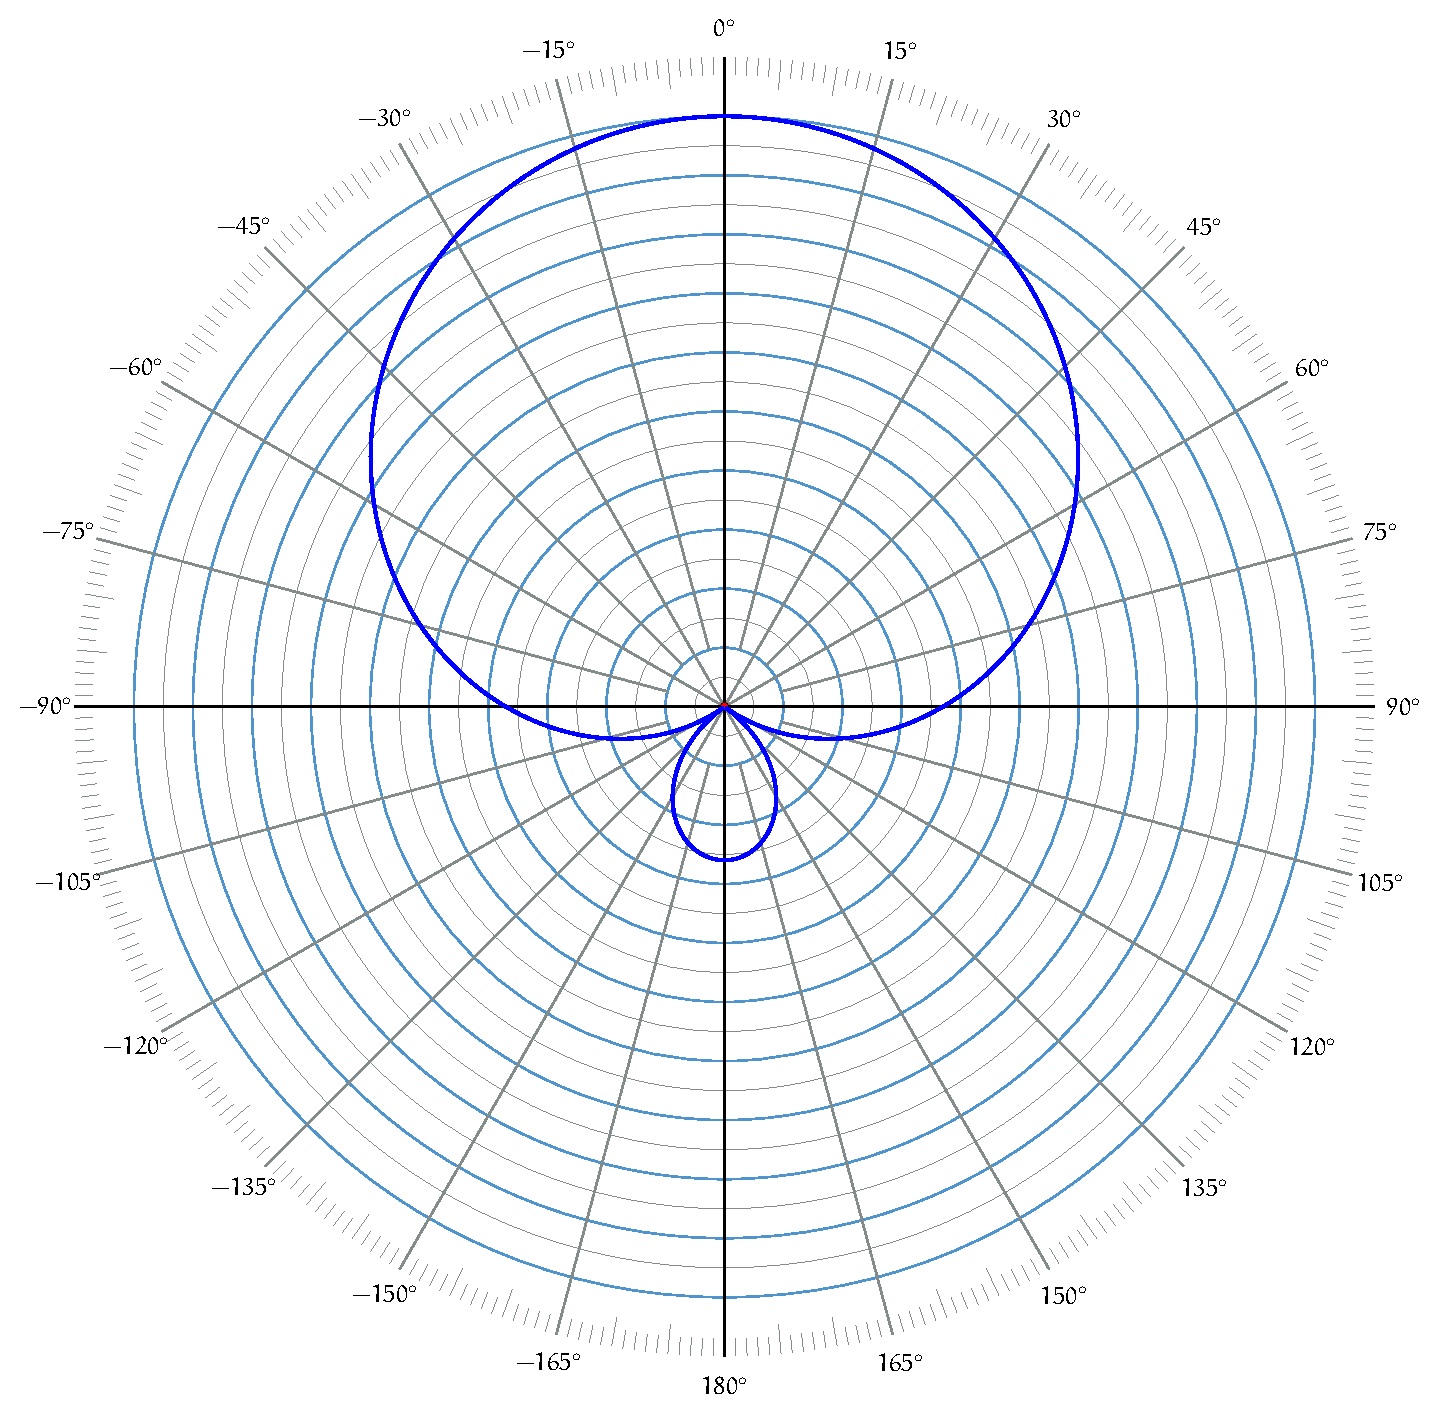
\includegraphics[width=\linewidth]{microphone-polar-patterns/supercardioid}\end{minipage}} \\
                & $0.37$       & $+$ & $0.63$               & \\
                & $-8.64dB$    & $+$ & $-4.01dB$            & \\ %20*log10(g)
& \\
\hline
ipercardioide   & $0.25(x)$    & $+$ & $0.75(x\cos\theta)$  &
 \multirow{4}{*}{\begin{minipage}{.25\textwidth}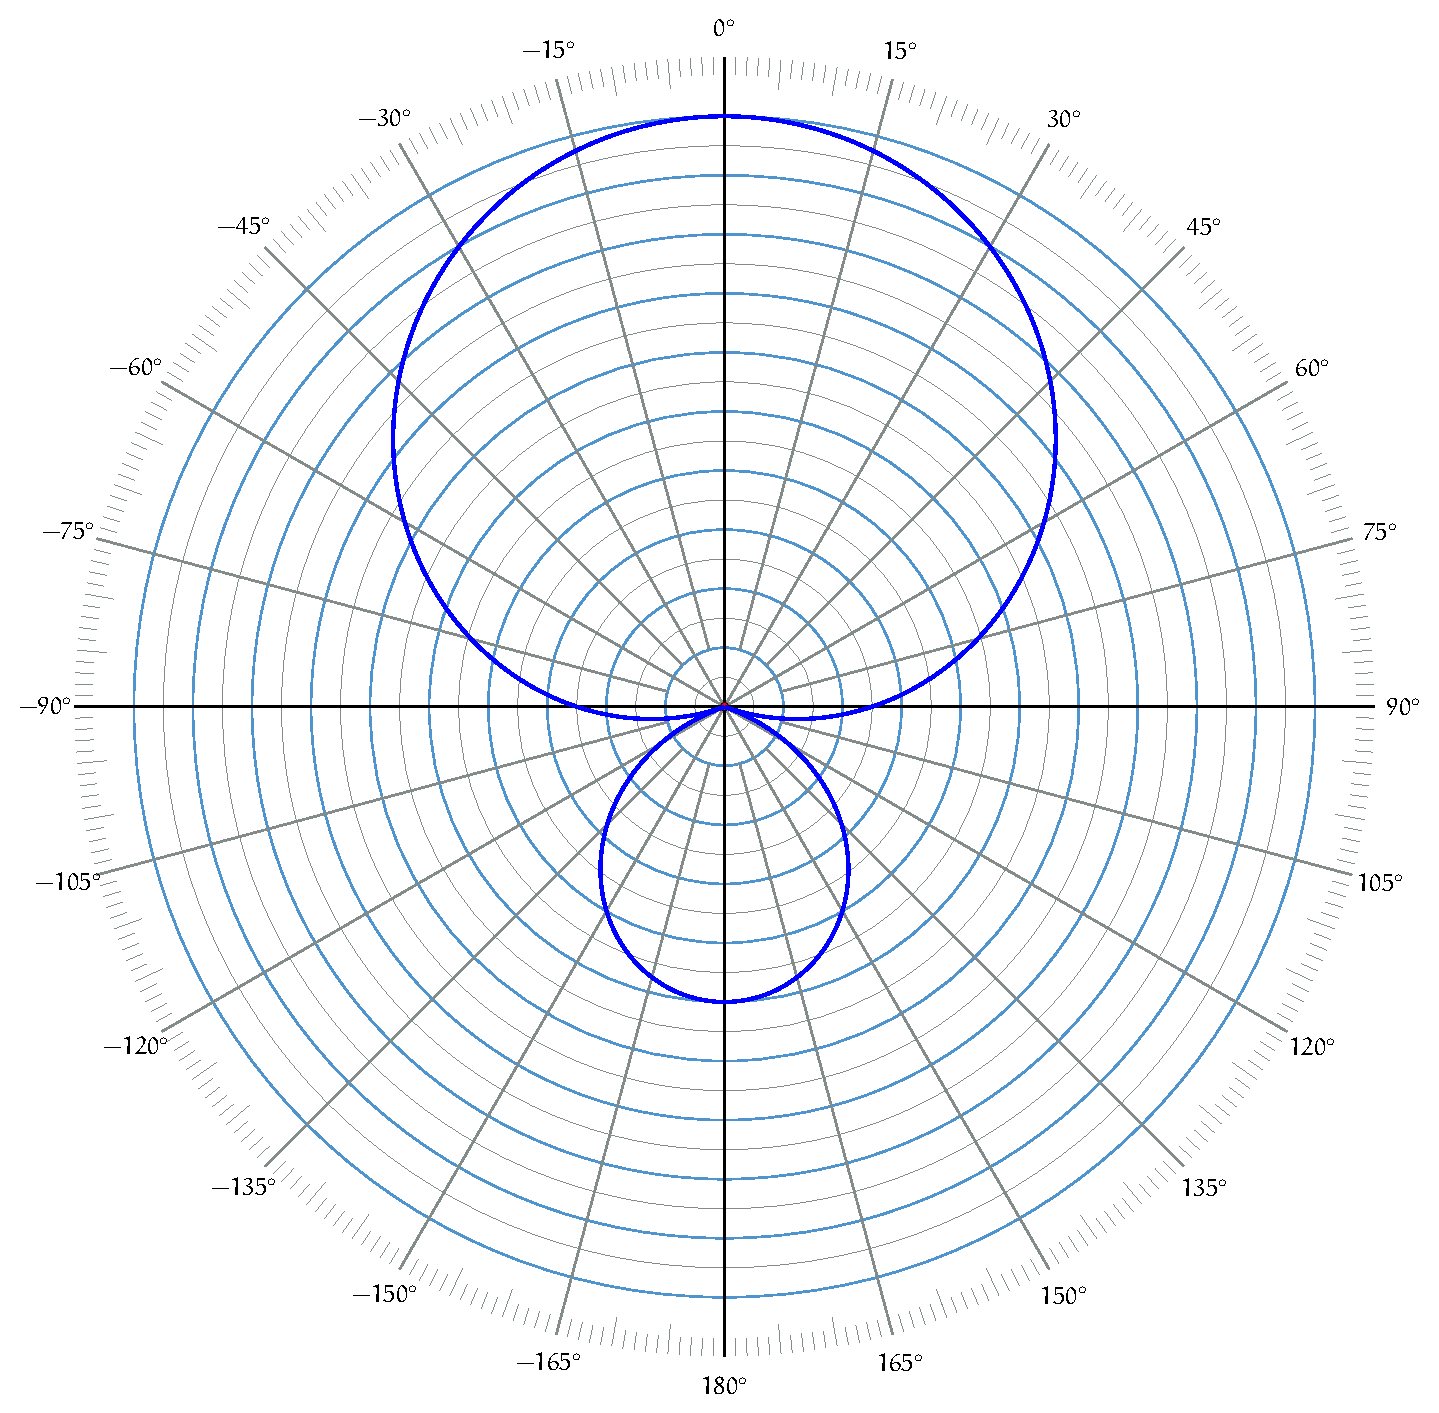
\includegraphics[width=\linewidth]{microphone-polar-patterns/hypercardioid}\end{minipage}} \\
                & $0.25$       & $+$ & $0.75$               & \\
                & $-12.05dB$ & $+$ & $-2.75dB$              & \\ %20*log10(g)
& \\
\hline
bidirezionale   &              &     & $1(x\cos\theta)$     &
 \multirow{4}{*}{\begin{minipage}{.25\textwidth}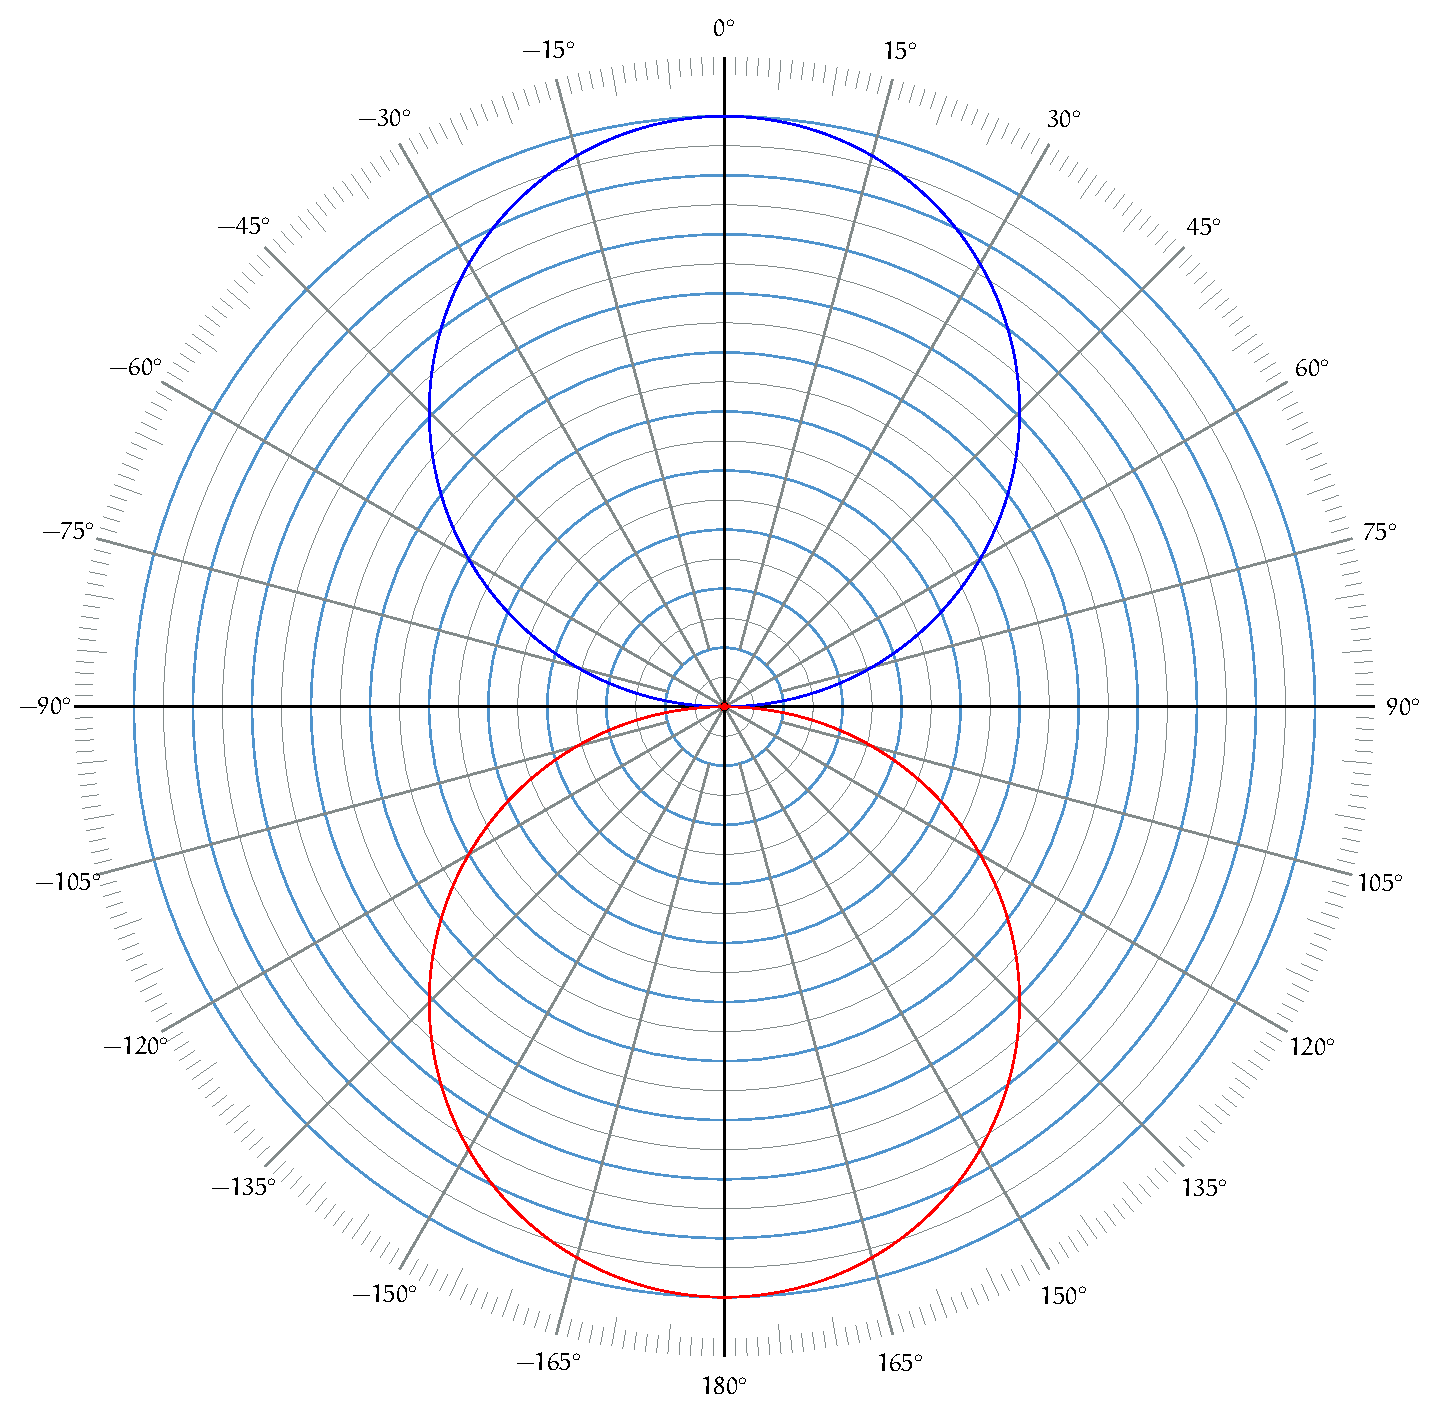
\includegraphics[width=\linewidth]{microphone-polar-patterns/fig8}\end{minipage}} \\
                & $0$          & $+$ & $1$                  & \\
                & $-\infty$    & $+$ & $0dB$            & \\ %20*log10(g)
& \\
\end{tabular}
\end{center}
\label{tab:polarcoef}
\end{table}

\clearpage

\begin{figure*}[h]
    \centering
    \begin{subfigure}[t]{0.48\textwidth}
        \centering
        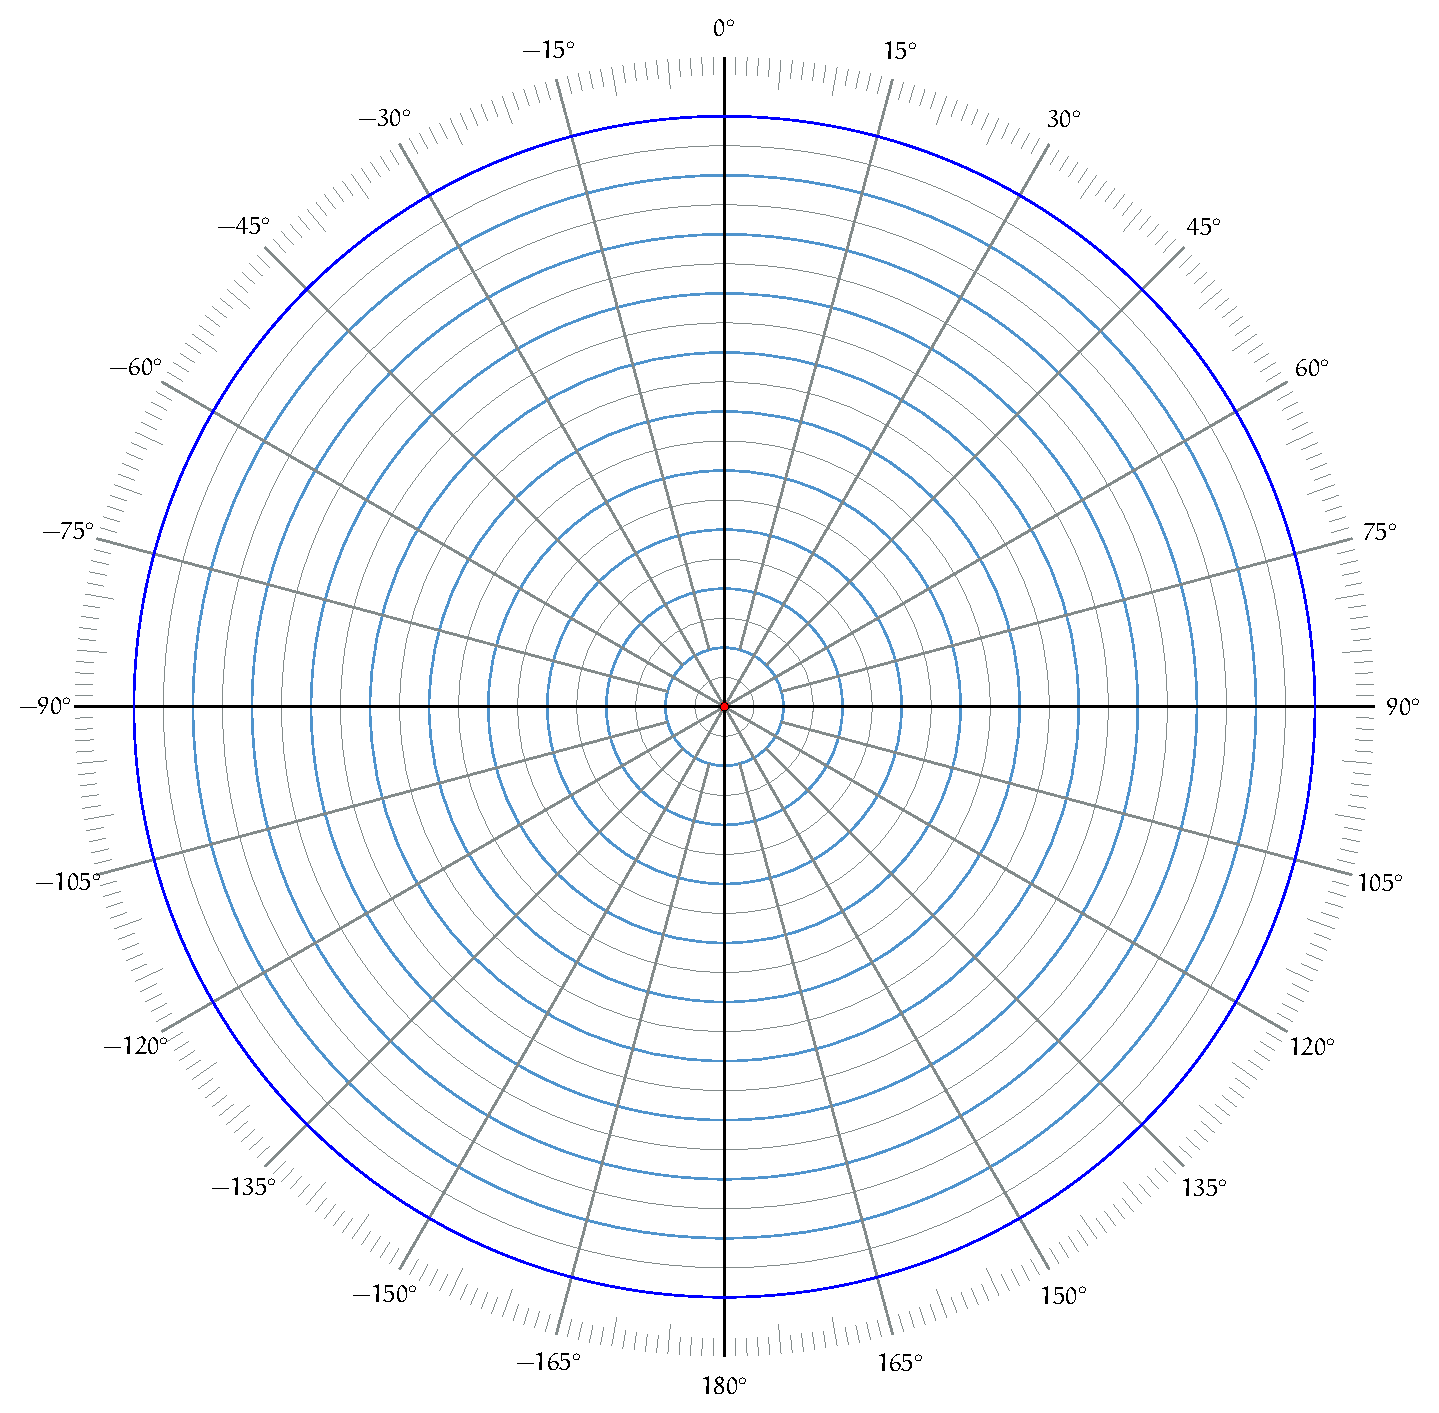
\includegraphics[height=6cm]{microphone-polar-patterns/omni}
        \caption[]{non-direzionale}% \\ Eq: $1(x)$}
        \label{pol:omni-p}
    \end{subfigure}%
    ~
    \begin{subfigure}[t]{0.48\textwidth}
        \centering
        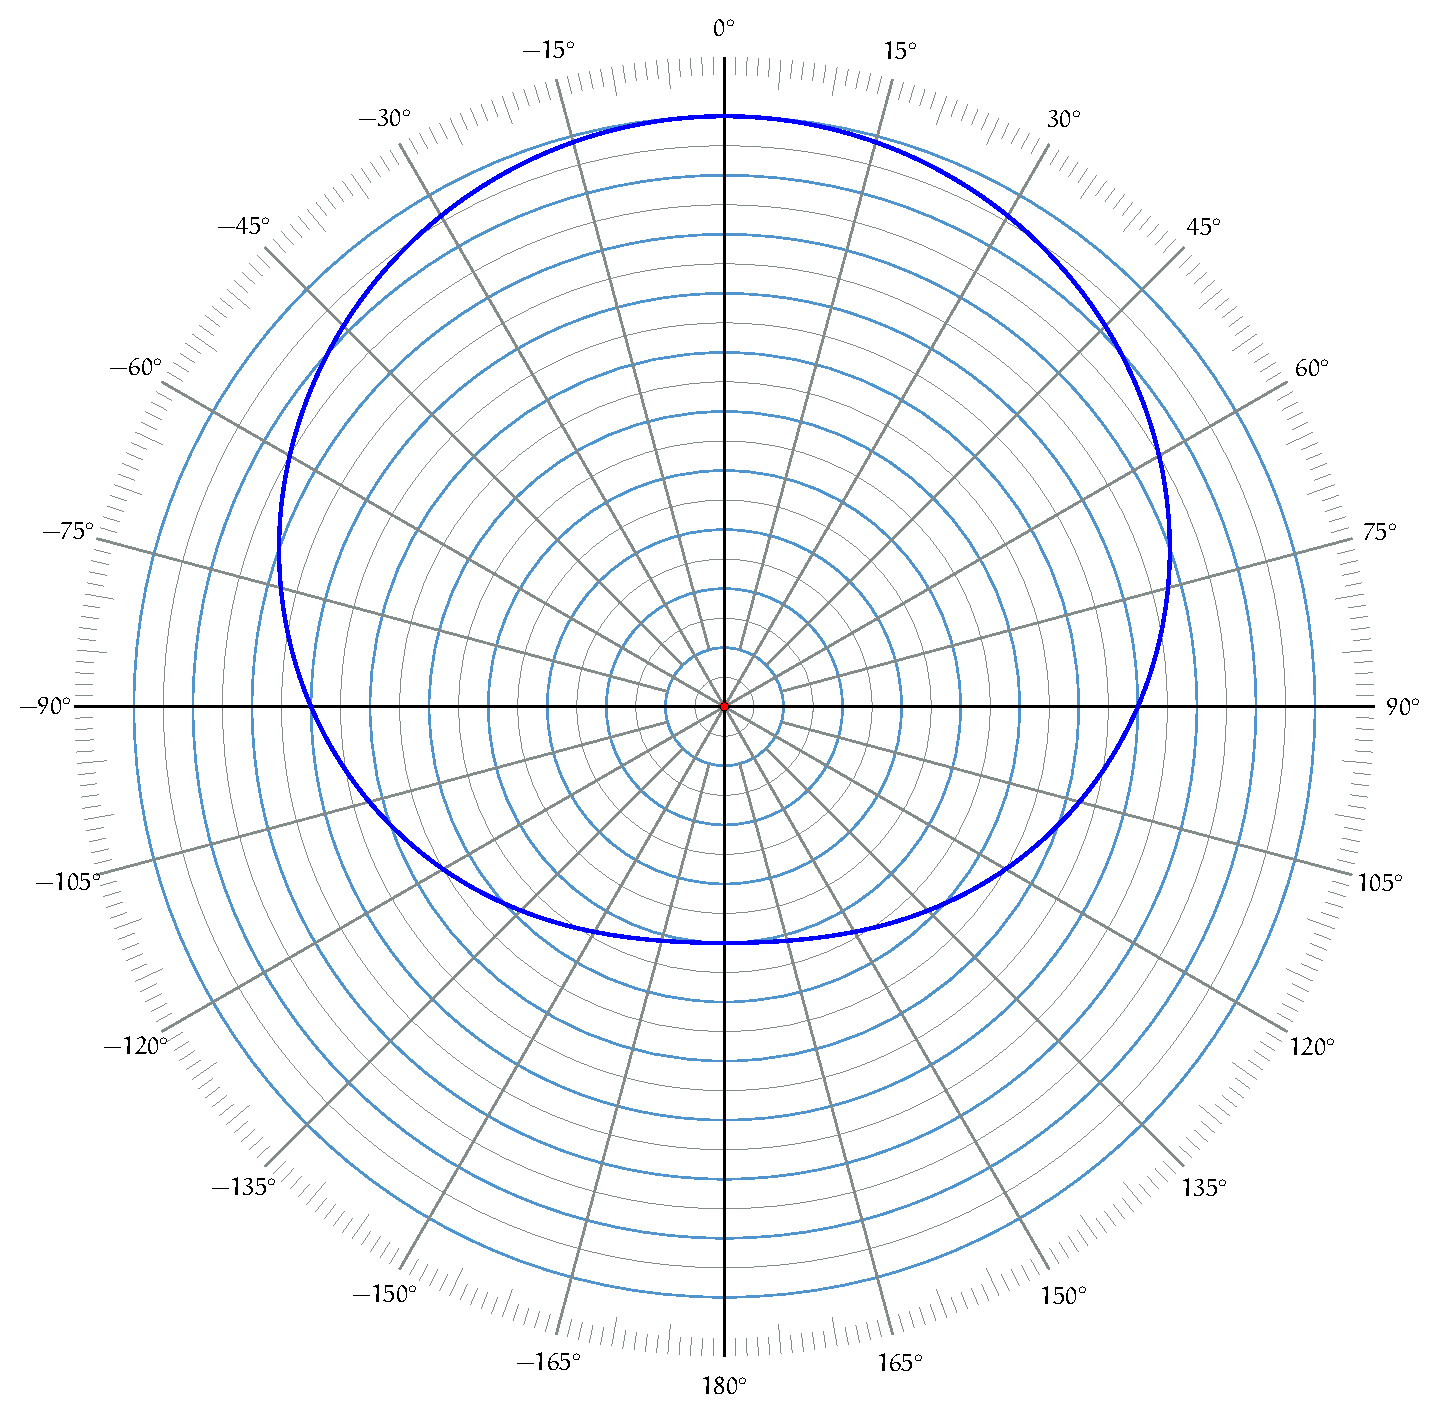
\includegraphics[height=6cm]{microphone-polar-patterns/subcardioid}
        \caption[]{subcardioide}% \\ Eq: $0.75(x)+0.25(x\cos\theta)$}
        \label{pol:sub-p}
    \end{subfigure}
    \\
    \begin{subfigure}[t]{0.48\textwidth}
        \centering
        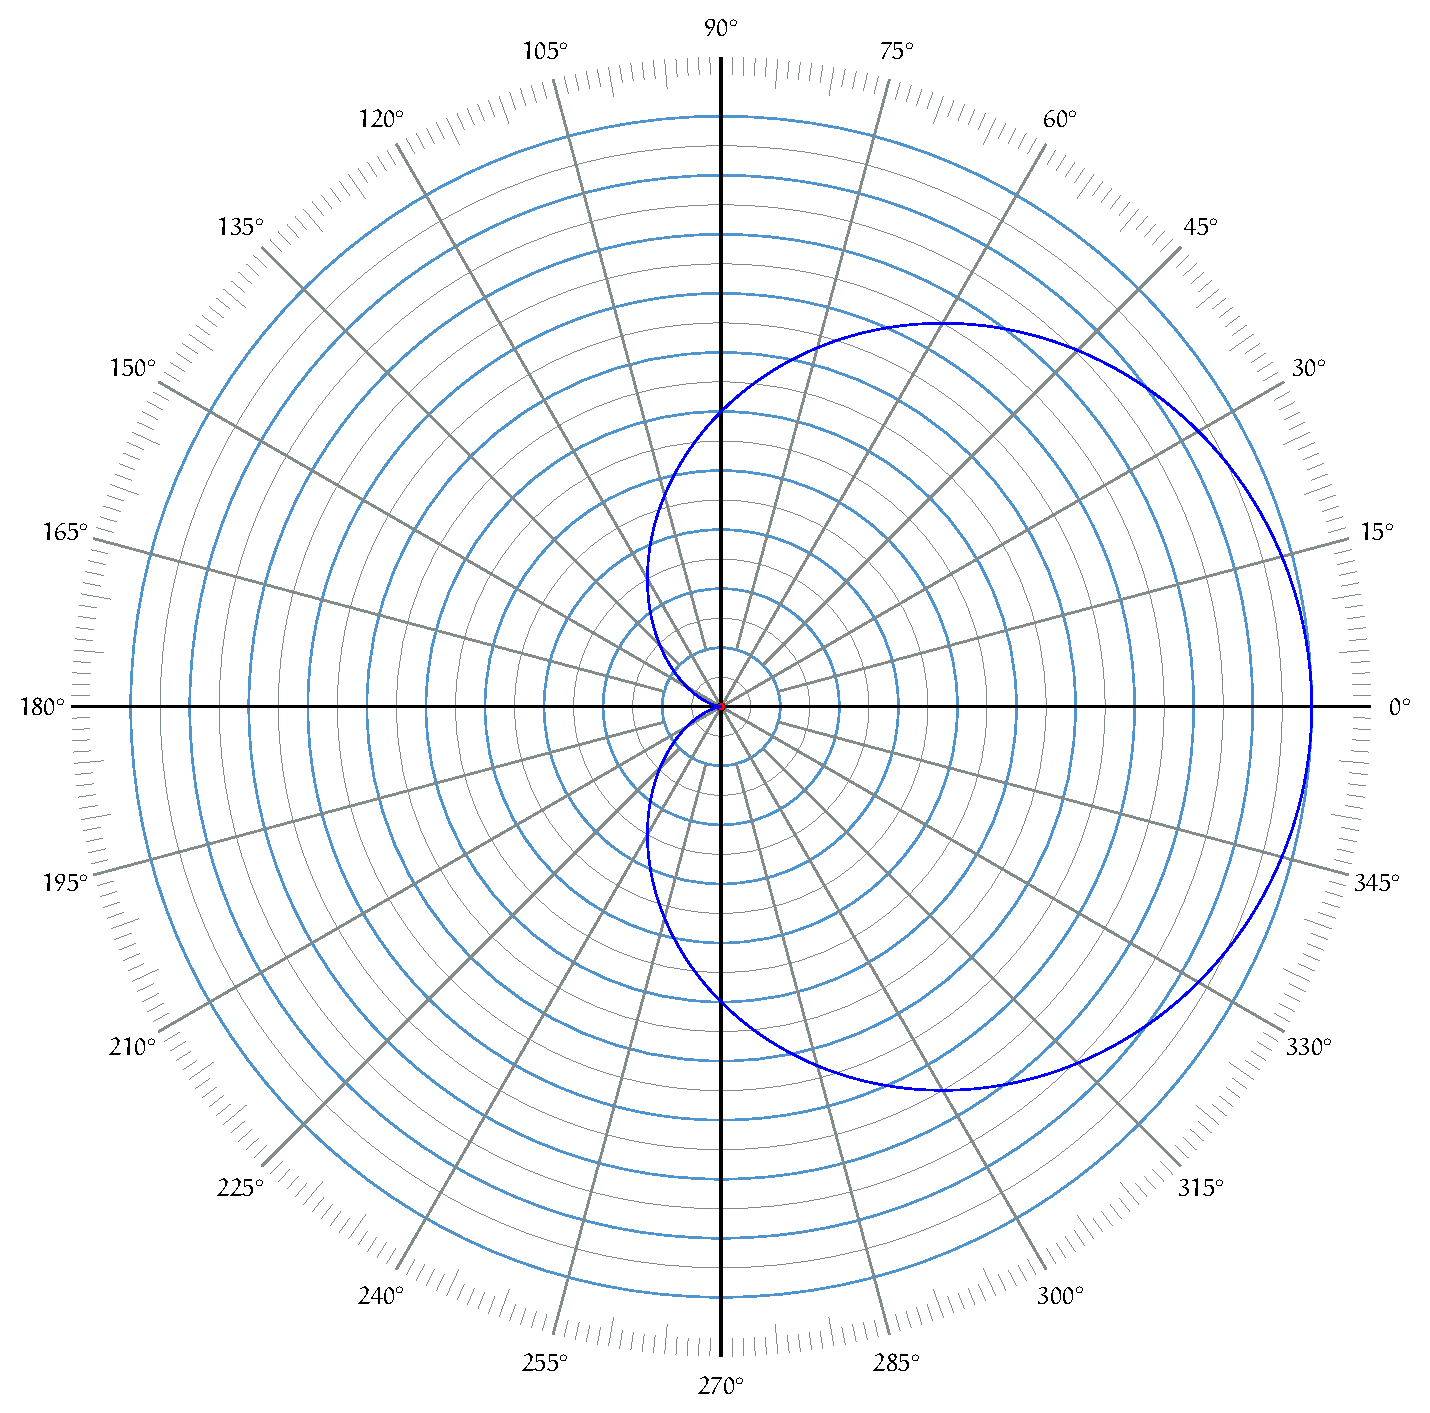
\includegraphics[height=6cm]{microphone-polar-patterns/cardioid}
        \caption[]{cardioide}% \\ Eq: $0.5(x)+0.5(x\cos\theta)$}
        \label{pol:cardio-p}
    \end{subfigure}
    ~
    \begin{subfigure}[t]{0.48\textwidth}
        \centering
        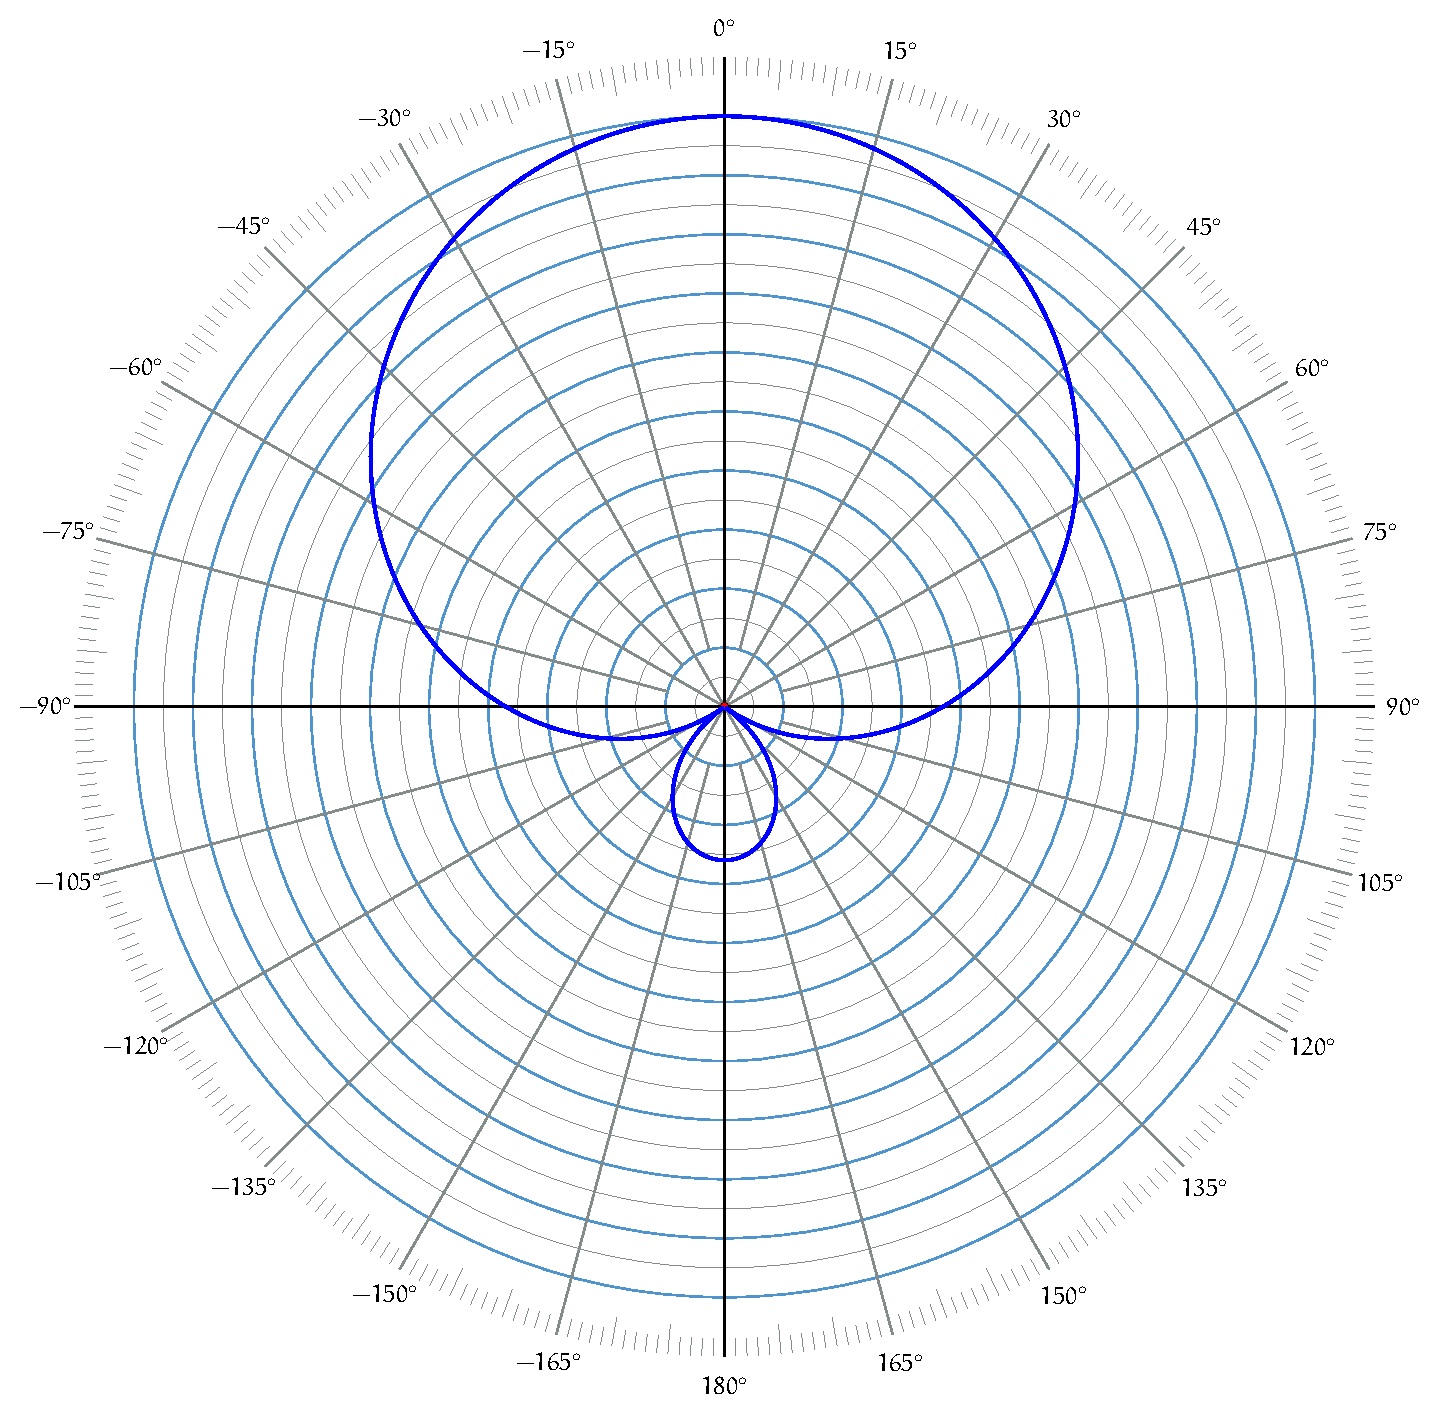
\includegraphics[height=6cm]{microphone-polar-patterns/supercardioid}
        \caption[]{supercardioide}% \\ Eq: $0.37(x)+0.63(x\cos\theta)$}
        \label{pol:super-p}
    \end{subfigure}
    \\
    \begin{subfigure}[t]{0.48\textwidth}
        \centering
        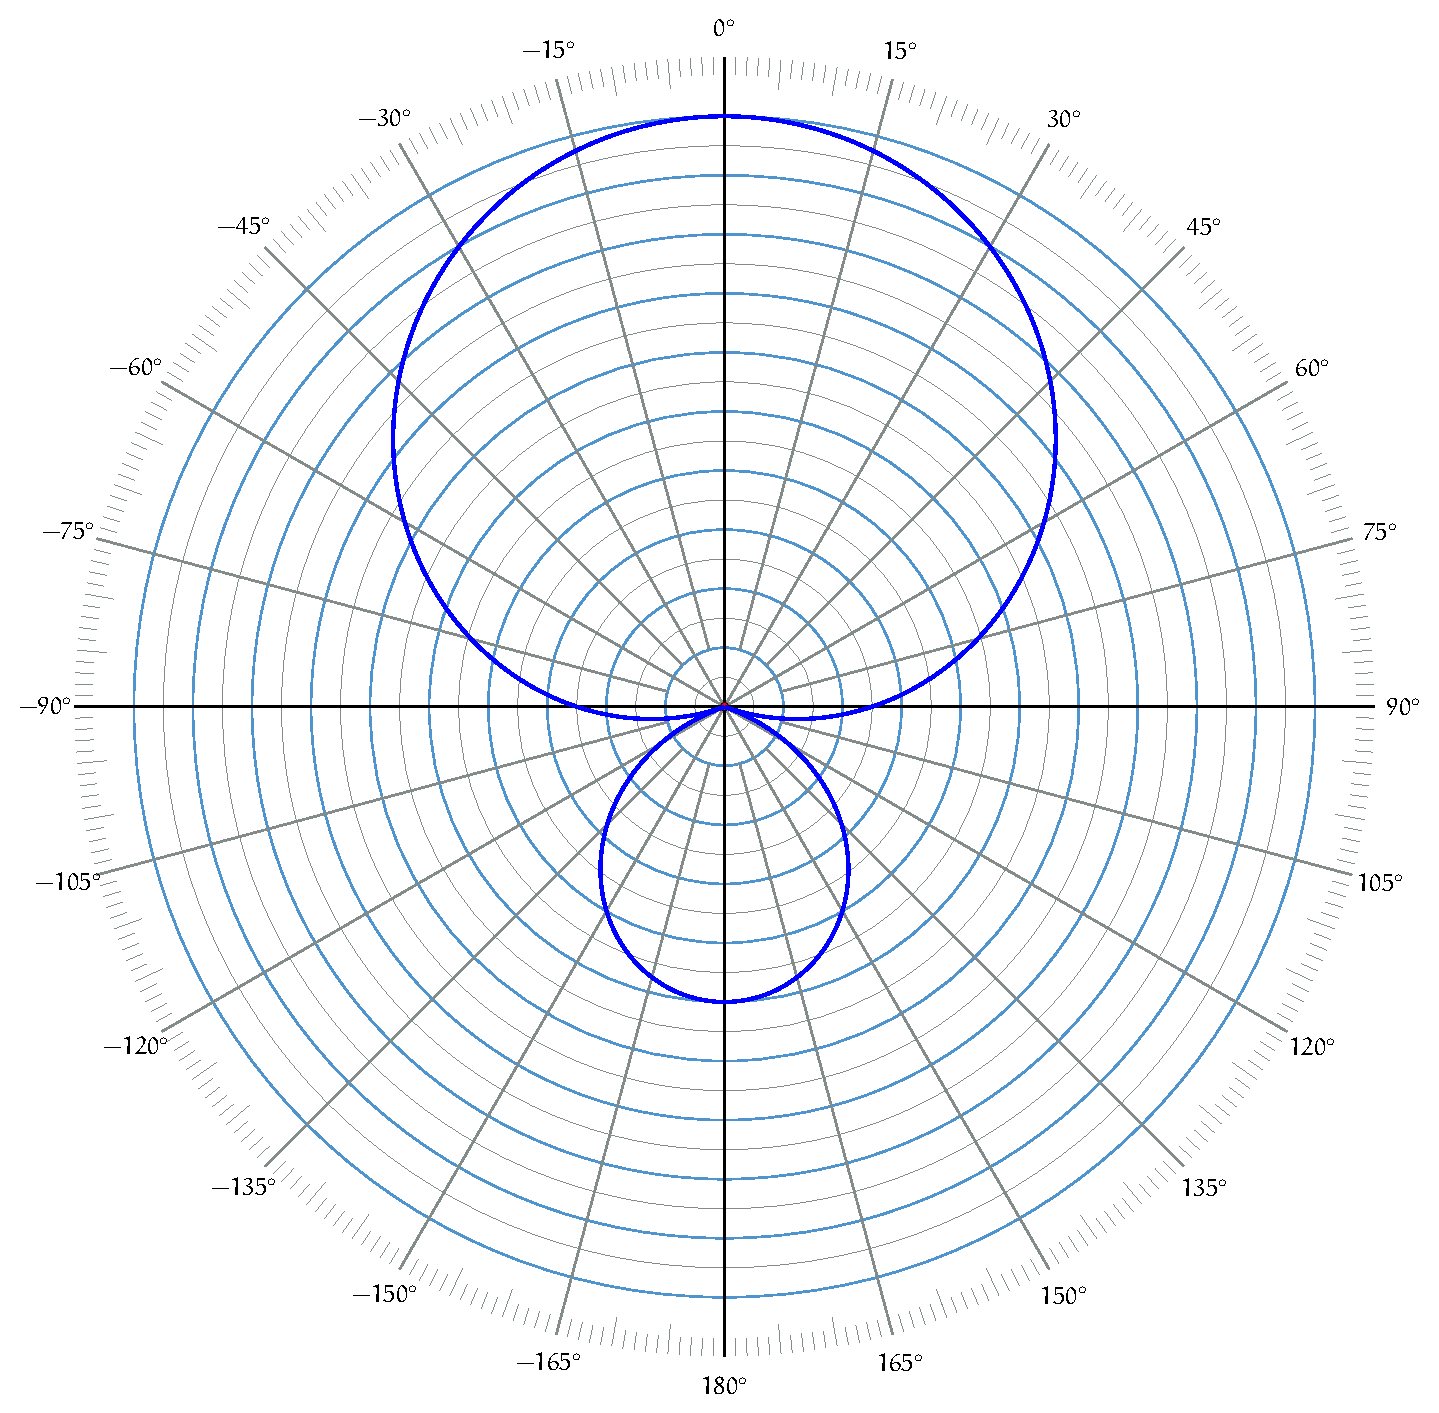
\includegraphics[height=6cm]{microphone-polar-patterns/hypercardioid}
        \caption[]{ipercardioide}% \\ Eq: $0.25(x)+0.75(x\cos\theta)$}
        \label{pol:iper-p}
    \end{subfigure}
    ~
    \begin{subfigure}[t]{0.48\textwidth}
        \centering
        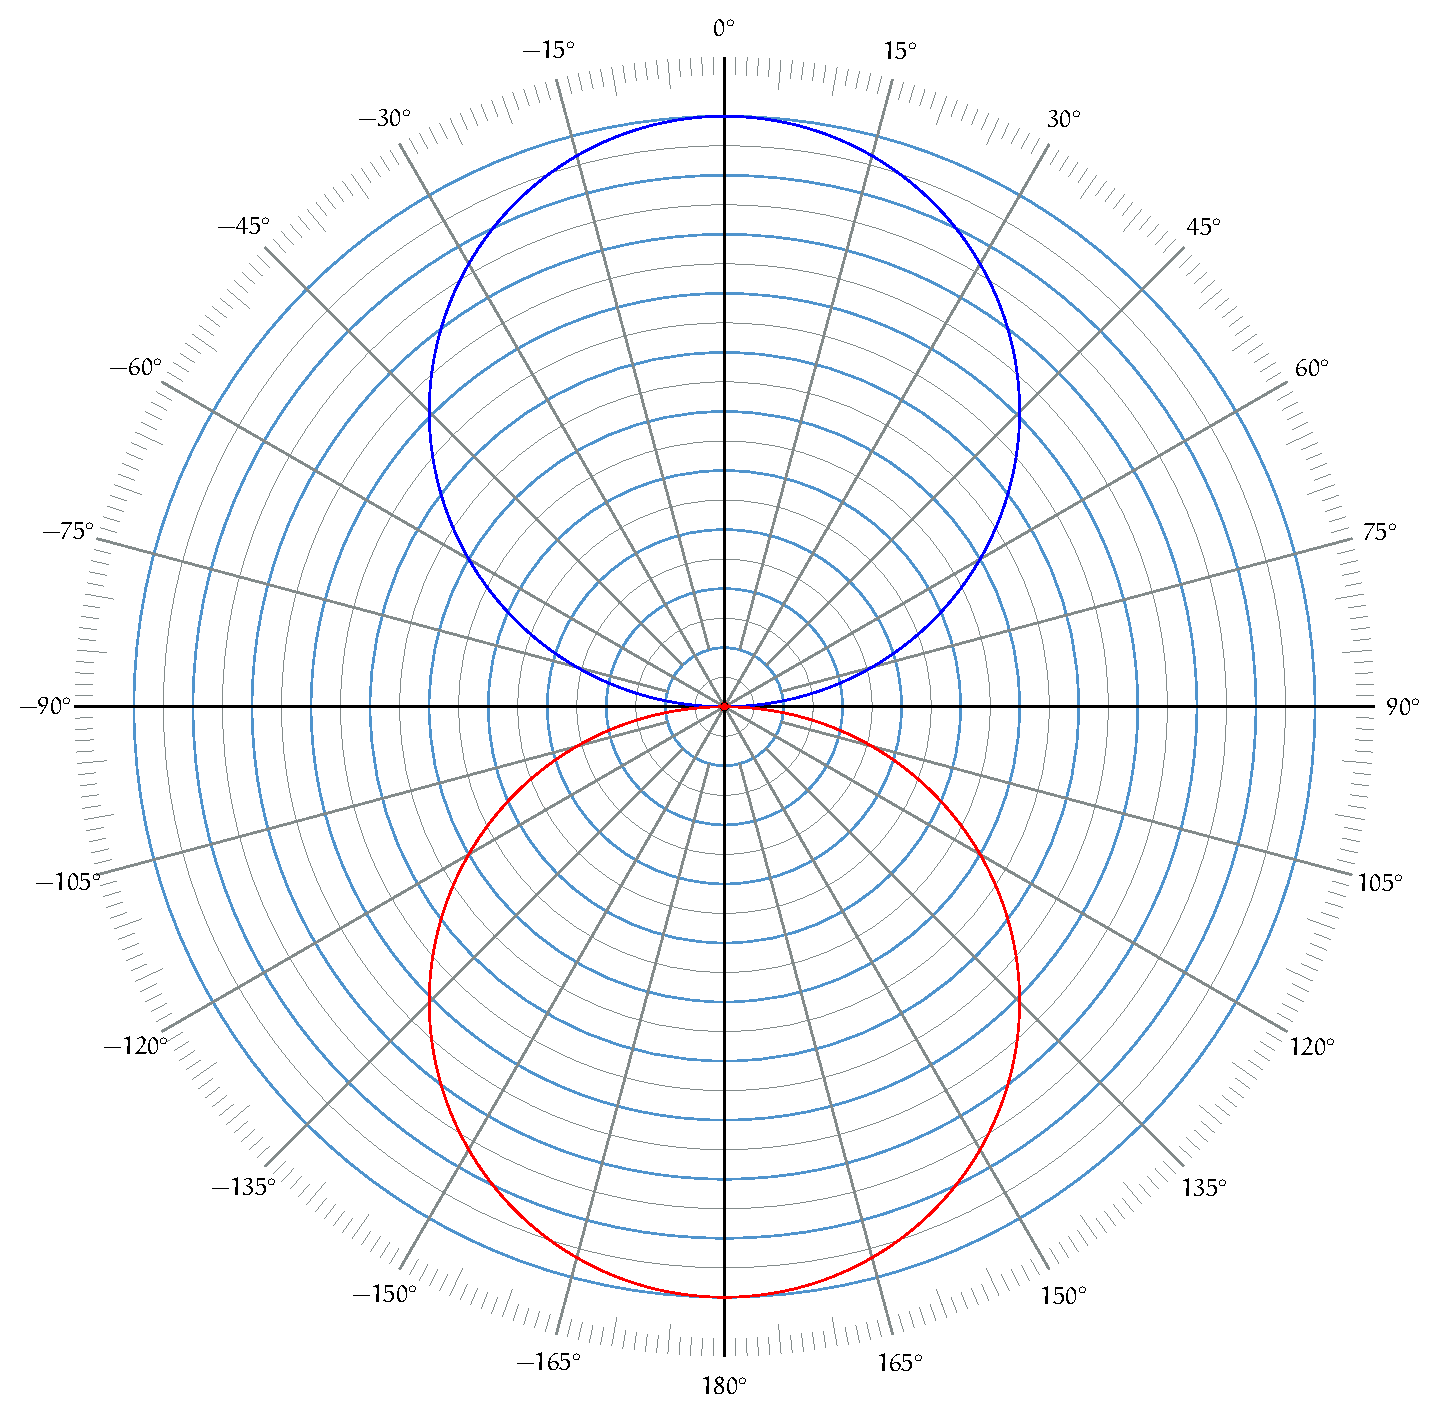
\includegraphics[height=6cm]{microphone-polar-patterns/fig8}
        \caption[]{figura-8}% \\ Eq: $1(x\cos\theta)$}
        \label{pol:fig8-p}
    \end{subfigure}
    \caption[]{Le principali figure polari ottenute mediante la calibrazione dei
    coefficienti di ampiezza della componente non-direzionale (fig. \ref{pol:omni-p}) e
    e bidirezionale (fig.\ref{pol:fig8-p}).}
    \label{pol:princicpali}
\end{figure*}

\printbibliography
\end{refsection}
